\documentclass[12pt]{article}
	\usepackage[T1]{fontenc}
	\usepackage[utf8]{inputenc}
	\usepackage[british]{babel}
	\usepackage[a4paper]{geometry}
	\geometry{verbose,tmargin=3cm,bmargin=3cm,lmargin=2cm,rmargin=2cm,marginparwidth=70pt}
	\setcounter{secnumdepth}{3}
	\setcounter{tocdepth}{2}
	\setlength{\parindent}{2em}
	\renewcommand{\baselinestretch}{1.5}
	\usepackage{prettyref}
	\usepackage{textcomp}
	\usepackage{booktabs}
	\usepackage{lscape}
	\usepackage{setspace}
	\usepackage{indentfirst}
	\usepackage{fancyhdr}
	\usepackage{url}
	\usepackage[normalem]{ulem}
	\usepackage[table, fixpdftex]{xcolor}
	\usepackage{algpseudocode}
	\usepackage{bigstrut}
	\usepackage{enumitem}
	\usepackage{verbatim}
	\usepackage{mathtools}
	\usepackage{graphicx}
	\usepackage{longtable}
	\usepackage{chngpage}
	\usepackage{pdfpages}
	\usepackage{rotating}
	\usepackage{adjustbox}
	\usepackage[toc,page,title]{appendix}
	\usepackage[super]{nth}
	\usepackage[all]{nowidow}
	\usepackage{ragged2e}
	\usepackage[font=scriptsize,labelfont=bf]{caption}
	\usepackage[nottoc]{tocbibind}
	\usepackage{glossaries}
	\usepackage{acro}
	\DeclareCaptionLabelFormat{blank}{}
	% package hyperref
    \usepackage[hidelinks]{hyperref}
  
	\urlstyle{same}
   
	% biblatex
	\usepackage[style=authoryear,natbib=true,maxcitenames=2,maxbibnames=11,backend=biber,pagetracker=page,hyperref=true,doi=true, mergedate=compact, firstinits=true]{biblatex} 
	\usepackage{csquotes}
	\renewcommand*{\bibsetup}{%
		\interlinepenalty=10000\relax % default is 5000
		\widowpenalty=10000\relax
		\clubpenalty=10000\relax
		\raggedbottom
		\frenchspacing
        \biburlsetup}
          
	% fixes the page number of the first page of each chapter
	\fancypagestyle{plain}{
			\fancyhead{}
			\renewcommand{\headrulewidth}{0pt}
			\renewcommand{\footrulewidth}{0pt}
			\fancyfoot[OC]{\begin{flushright}\thepage\end{flushright}}
    }
    
	% fancy headers for the thesis
	\fancyhead{}
	\fancyhead[RO]{\slshape \nouppercase \rightmark}
	\fancyfoot[OC]{\begin{flushright}\thepage\end{flushright}}
	\renewcommand{\headrulewidth}{0.4pt}
	\setlength{\headheight}{14pt}


	% add bibliography database
	\addbibresource{BA copy.bib}
	
	% space between biblio items
	\setlength\bibitemsep{1.7\itemsep} 
	
	% title without ""
	\DeclareFieldFormat[inbook]{title}{#1}
	% non-italic
	\DeclareFieldFormat[online]{tlaitle}{#1} 
	% title unquoted
	\DeclareFieldFormat[article]{title}{#1} 
	% no pp. 
	\DeclareFieldFormat[article]{pages}{#1} 
	% bold volume
	\DeclareFieldFormat*{volume}{\mkbibemph{#1}\setpunctfont{\textit}}
	
	% no in:
	\renewbibmacro{in:}{} 
	
	% (volume)
	\renewbibmacro*{volume+number+eid}{%
			\printfield{volume}%
			%\setunit*{\adddot}% DELETED
			% \setunit*{\addnbspace}% NEW (optional); there's also \addnbthinspace
			\printfield{number}%
			% \setunit{\addcomma\space}%
			\printfield{eid}}
	\DeclareFieldFormat[article]{number}{\mkbibparens{#1}} 
	
	% edition.
	\DeclareFieldFormat{edition}%
	{(\ifinteger{#1}%
			{\mkbibordedition{#1}\addthinspace{}ed.}%
			{#1\isdot}).}
	
	% publisher and location position
	\renewbibmacro*{publisher+location+date}{%
			\printlist{publisher}%
			\setunit*{\addcomma\space}%
			\printlist{location}%
			\setunit*{\addcomma\space}%
			\usebibmacro{date}%
			\newunit}
	
	% shortauthor before author
	\renewbibmacro*{begentry}{%
			\ifkeyword{Key}{\sffamily}{}%
			\iffieldundef{shorthand}
			{}
			{\global\undef\bbx@lasthash
					\printfield{shorthand}%
					\addcolon\space}%
			\ifboolexpr{test {\usebibmacro{bbx:dashcheck}} or test {\ifnameundef{shortauthor}}}%
			{}%
			{\printnames{shortauthor}%
                    \addspace\textendash\space}}

\AtBeginBibliography{%
  \renewcommand*{\finalnamedelim}{%
    \ifnumgreater{\value{liststop}}{2}{\finalandcomma}{}%
    \addspace\&\space}%
}
\DeclareNameAlias{sortname}{last-first}

\DefineBibliographyStrings{english}{%
    url = {Retrieved from}
}
\DeclareFieldFormat{url}{\bibstring{url}\space\url{#1}}

%List of Abbreviations
\makeatletter
\newcommand{\tocfill}{\cleaders\hbox{$\m@th \mkern\@dotsep mu . \mkern\@dotsep mu$}\hfill}
\makeatother

\newcommand{\abbrlabel}[1]{\makebox[7cm][l]{#1\ \dotfill}}
\newenvironment{abbreviations}{\begin{list}{}{\renewcommand{\makelabel}{\abbrlabel}\setlength{\labelwidth}{7cm}\setlength{\leftmargin}{\labelwidth+\labelsep}%
\setlength{\itemsep}{0pt}}}{\end{list}}

\title{Does Financial Constraints of Corporate Activist Investors Matter?}
\author{Leopold Ingenohl}

\newcounter{savepage}
\begin{document}

\begin{titlepage}
    \begin{center}
       
        
\includegraphics[width=0.5\textwidth]{Logo.jpg}
       
        \vspace*{1.5cm}
		\Large
        \textbf{Do Financial Constraints of Corporate Activist Investors Matter?}

        \vspace{1.5cm}
		\normalsize
        Leopold Ingenohl\\
        Richard-Wagner Str. 7\\
        76185, Karlsruhe\\
        leopold.ingenohl@student.unisg.ch\\
        15-613-631

        \vspace{1.5cm}
        Supervised by\\
        Prof. Dr. Markus Schmid\\
        Swiss Institute of Banking and Finance (s/bf)\\
        \vfill

        A thesis presented for the degree of\\
        Bachelor of Arts HSG

        \vspace{0.8cm}

        Submitted May 22, 2018

	\end{center}
	
\end{titlepage}

\cleardoublepage
\pagenumbering{roman}
\begin{abstract}
\noindent To analyze whether financial constraints of corporate activist investors matter, this thesis investigates the relationship between financial constraints of corporations disclosing a Schedule 13(D) filing, and the resulting abnormal returns to the targets. By using a sample of 561 Schedule 13(D) filings disclosed by corporations in the years from 1996-2016 in the United States and conducting an event study, abnormal share price reactions surrounding the filing date identify the effect the Schedule 13(D) filing has on the target's stock. In fact, estimating abnormal returns via the market model results in average cumulative abnormal returns of 13.3\% for all targets in the event-window [-10,3]. The positive market response is consistent with the evidence on the market’s perception that activism results in actual value improvement for the target. Further, using a variety of financial constraints measures, the investing corporations are classified into groups of financially constrained and unconstrained investors. The univariate analysis shows that targets of financially constrained investors experience significantly lower abnormal returns in response to Schedule 13(D) filings, with average cumulative abnormal returns around 10\% lower in a [-10,3] event window. Both, across different transaction purposes and measures of financial constraints is the difference apparent. The multivariate analysis confirms that, other things equal, targets of financially constrained investors experience lower abnormal returns when compared to targets of unconstrained investors. This proves a negative relationship between targets' abnormal returns and investors' financial constraints. The evidence allows to draw the conclusion, that financial constraints of corporate activist investors matter.
\end{abstract}

\pagebreak
\renewcommand{\baselinestretch}{1.5}\normalsize
\renewcommand{\contentsname}{Table of Contents}
\tableofcontents
\cleardoublepage
\listoftables
\listoffigures
\renewcommand{\baselinestretch}{1.5}
\section*{List of Abbreviations}
\addcontentsline{toc}{section}{List of Abbreviations}
\begin{abbreviations}
	\item[AT] Total Assets
	\item[AMEX] American Stock Exchange
	\item[AR] Abnormal Returns
	\item[BHAR] Buy-and-hold Abnormal Return
	\item[CAR] Cumulative Abnormal Return
	\item[CEO] Chief Executive Officer
	\item[CIK] Central Index Key
	\item[CRSP] Center for Research in Security Prices
	\item[CUSIP] Code derived from the Committee on Uniform Security Identification Procedures which identifies a North American financial security
	\item[Dif.] Difference
	\item[EBITDA] Earnings Before Interest and Taxes
	\item[EDGAR] Electronic Data Gathering, Analysis, and Retrieval system
	\item[FC] Financially Constrained
	\item[GVKEY] Global Company Key -- Unique Six-Digit Number Key Assigned to Each Company in the Compustat Database
	\item[HP-Index] Hadlock-Pierce Index
	\item[$H_{A}$] Alternative Hypothesis 
	\item[$H_{0}$] Null Hypothesis 
	\item[KZ-Index] Kaplan-Zingales Index
	\item[Max.] Maximum
	\item[Med.] Median
	\item[Min.] Minimum
	\item[N] Number of Observations
	\item[NASDAQ] National Association of Securities Dealers Automated Quotations
	\item[NYSE] The New York Stock Exchange
	\item[p.] Page
	\item[PERMNO] Unique Permanent Security Identification Number assigned by CRSP to each Security
	\item[ROA] Return on Assets
	\item[SA-Index] Size-Age Index
	\item[SEC] Securities and Exchange Commission
	\item[SIC] Standard Industry Classification
	\item[S\&P] Standard \& Poor's
	\item[Std. Dev.] Standard Deviation
	\item[U.S.] United States
	\item[WRDS] Wharton Research Data Services
	\item[WW-Index] Whited-Wu Index
\end{abbreviations}

\renewcommand{\baselinestretch}{1.5}\normalsize
\cleardoublepage
\setcounter{savepage}{\arabic{page}}
\pagenumbering{arabic}


\section{Introduction}

\noindent If any person acquires beneficial ownership of more than 5\% of an issuer's securities in the United States, he must file with the Securities and Exchange Commission (SEC) a Schedule 13(D), within 10 days after the acquisition of that stock. The crux herein lies in beneficial ownership, which is not defined as whether the person owns the shares but as whether the particular person can vote the shares and thereby change or influence the control of the company \citep[p.24]{Morrison2015}. Precisely, this mindset is what constitutes shareholder activism, independent of the acquirers identity. In fact, a Schedule 13(D) has to be disclosed by most investor types such as individuals, hedge funds and corporations. In the words of \citet[p.187]{Klein2009}, an "entrepreneurial activist is an investor who buys a large stake in a publicly held corporation with the intention to bring about change and thereby realizes a profit on the investment". Complementary thereto, corporations filing a Schedule 13(D) to deliberately engage in their investment, can be classified as corporate activist investors.\par
Hedge fund activists seek to gain seats on the company's board, oppose an existing merger or liquidation of the firm, pursue strategic alternatives or replace the CEO \citep[p.188]{Klein2009}. Motivation for corporate activist investors to acquire beneficial ownership is to overcome informational and integration barriers and thereby engage in proceedings such as takeovers and strategic cooperations \citep[p.1]{Huang2017}. Strategic minority acquisitions help reduce holdup costs, mitigate financing constraints and facilitate greater innovation and relation-specific investment \citep[p.825]{Wang2014}. In turn, they are followed by significant benefits for both firms \citep[p.2793]{Allen2000}.\par
This action for change is mirrored by a positive market response at the announcement of the filing. Hence, when an investor's Schedule 13(D) filing becomes public, the firm that has been partially acquired experiences significant gains on its stock. In recent studies of what happens to the target's stock, \citet[p.1564]{Collin-Dufresne2015} find significant positive abnormal returns around the filing day for filings of all investor types. The evidence is consistent with \citet[p.1756]{Brav2008} and \citet[p.209]{Klein2009} who report 8.4\% and 7.2\% abnormal returns respectively but in response to hedge fund activism. The only study inexplicitly noting a positive market response to corporate Schedule 13(D) filings is by \citet[p.29]{Brigida2012}. This thesis fills the present shortage and finds evidence that targets of corporate activist investors experience positive abnormal returns around the filing date of the Schedule 13(D). In fact, estimating abnormal returns via the market model results in average cumulative abnormal returns of 13.3\% for all targets in the event-window [-10,3]. The positive market response is consistent with the evidence of the market's perception that activism, likewise action for change, results in actual value improvement for the target \citep[p.1760]{Brav2008}.\par
The potential increase in value however, is dependent on the initiators of activism, as it is their own effort that brings the change \citep[p.1563]{Collin-Dufresne2015}. So if the initiator of activism stands for the actual value improvement, its ability to finance action for change and further involvement in the target, hence its financial appearance, should be related to the market's evaluation of the target's potential gains.\par
A recent example on this matter is the public's perception of China's largest private conglomerate, the HNA Group. Over the past few years they invested around \$US40 billion in businesses around the world and have currently been of great interest to financial news \citep{Smith2018}. Not least because they built up a 9.9\% stake of around \$US4 billion in Deutsche Bank in 2017, but also because of their complex and nontransparent financing methods \citep{Lockett2018}.
The financing of the group has come under strain as a result of an official crackdown on risky financing of acquisitive private enterprises in China. The highly leveraged group is now facing a potential cash-shortfall and liquidity issues resulting in a S\&P global rating downgrade referring to a a „deteriorating liquidity profile" of HNA \citep{Schuetze2018}. Although the HNA Group is a private conglomerate, the financial appearance of the investor seems to be of great interest to other market participants. The Schedule 13(D) on 28 April, 2018 in which they announced their 9.9\% stake in Deutsche Bank was followed by an increase in Deutsche Bank's value. This said, had the increase in value of Deutsche Bank been larger with an HNA Group financially less constrained and thereby more assertive? Hence do financial constraints of corporate activist investors matter?\par
As financially unconstrained corporations are able to raise substantial amounts of external capital, thereby signalizing the capability to bring potential change, the opposite should be true for financially constrained firms \citep[p.272]{Farre-Mensa2016}. If further the assumption holds that the actual value improvement for the target is dependent on the ability of the investor to bring change, the perceived value improvement for the target -- represented by abnormal returns -- should be smaller for those of financially constrained investors.\par 
This thesis finds evidence that it does. The univariate tests show that targets of financially constrained corporations gain less when compared to targets of unconstrained investors. For instance, when financially constrained investors are identified by using the Whited-Wu index, the target's abnormal return is on average 10\% higher had they been unconstrained. They have average abnormal returns of around 6\% whereas targets of financially unconstrained firms experience average abnormal returns of around 16\%. The significant difference of 10\% in abnormal returns indicates that financial constraints of corporate activists investors matter. The difference is also apparent across all transaction purposes, further supporting the proposition that financial constraints generally matter. The multivariate analysis confirms that, other things being equal, the financial constraints of the investor are an important determinant of the abnormal returns of the target. Targets of constrained investors earn 10\% less in the [-10,3] event-window indicating financial constraints of corporate activist investors matter, when the market perceives the actual value improvement for the target.\par
The paper proceeds as follows. Section 2 reviews relevant literature on Schedule 13(D) filings, their effect on the market, corporate equity ownership and financial constraints. Section 3 introduces the measures of financial constraints, outlines the composition of the sample and identifies the sample's corporate activist investors. Section 4 investigates the market's reaction to Schedule 13(D) filings and analyses the univariate relation between target's abnormal returns and investor's financial constraints. Following the univariate analysis, Section 5 evaluates the cross-sectional effect financially constrained investors have on the target's gains.

\section{Literature Review}

\subsection{Schedule 13(D) Filings \& Abnormal Returns}
%Topics: Historical Background | Information contained | Difference G and D

\noindent Section 13(d) of the Exchange Act of 1934 was passed in order to increase regulation of tender offers and accumulations of stock.
It acts as an early warning, signaling "every large, rapid aggregation or accumulation of securities, regardless of technique employed, which might represent a potential shift in corporate control" \citep[p.2]{Morrison2015}. This means that under Section 13(d), anyone who becomes the beneficial owner of 5\% of an issuer's equity securities registered under Section 12 of the Exchange Act must file with the SEC a Schedule 13(D) within 10 days after the acquisition. The filing informs shareholders about investors who could influence or change control of the issuing company \citep[p.110]{Giglia2016}. The investors filing such a Schedule 13(D) can be broadly classified into institutional investors (e.g. hedge funds or mututal funds), other entrepreneurial activists (e.g. individual investors) \citep[p.188]{Klein2009} and relevant for this thesis, corporate investors. Amongst others, the filing specifies the security and the issuer subject to the filing, the identity and background of the filer, and the purpose of the transaction.\par
Whereas filing a Schedule 13(D) allows the investor to practice its voting power in an active manner, a passive investor can equivalently file a Schedule 13(G). It is a short-form filing that can be utilized if an investor holds a beneficial ownership interest passively, with no intent to change control of the company \citep{Giglia2016}. Therefore, corporations filing a Schedule 13(D) confess to manage their investments actively, likewise confess to approach and interact with the target company and can therefore be called corporate activist investors.\par
So far, there exist many studies that examine the effect the disclosure of such an activist investment has on the target's stock. With regards to short-horizon event studies, all these studies find positive and significant abnormal returns around the Schedule 13(D) filing date. 
Dealing with investor activism, especially filings disclosed by hedge funds, \citet[p.1730]{Brav2008} find positive average abnormal returns in the range of 7\% to 8\% in the (-20,+20) event window. \citet[p.188]{Klein2009} have similar findings and observe 10.2\% average abnormal stock returns on the target's stock. In a more recent study on investor activism by \citet[p.410]{Denes2017}, the average valuation effect is evaluated to be around 5\%. 
A somewhat different approach is found in a study of \citet[p.363]{Greenwood2009} who observe abnormal announcement returns of 2.36\% for a sample of activist portfolio investors but document that the ability to force the target into a takeover is the driving force behind the abnormal market response. Nevertheless, all studies observe positive abnormal returns around the filing date and results primarily differ in magnitude.\footnote{Comparing the average abnormal returns across studies can be misleading as the authors use different models and event windows for estimating and aggregating the abnormal returns. \citet{Greenwood2009} use the market return model with matching portfolios and aggregate over [-10,5]; \citet{Brav2008} calculate the aggregated abnormal returns by subtracting the value-weighted market index from the buy-and-hold return and aggregate over a [-20,20] window; \citet{Klein2009} use a similar approach with the buy-and-hold returns but make several adjustments and aggregate over a [-30,5] window.}\par
While all of these studies identify hedge fund activism, its motivation and the effect it has on the market, most of them leave filings submitted by corporations aside. \citet[p.29]{Brigida2012} however, note that if the acquirer is a non financial corporation abnormal returns in the (-10,-1) window are around 14\%. The reaction implies the market perceives such corporate investments as value generating for the target. \citet[p.2803]{Allen2000} find abnormal returns of around 7\% in the (-10,10) period on corporate purchase announcements which are significantly larger if the announcement is accompanied by strategic investments. Their sample however is based on purchase announcements and therefore differs from studies on the effect of Schedule 13(D) filings.\footnote{In \citet[p.2801]{Allen2000} sample, the mean fraction of equity acquired in the sample is 14\%, and  only includes acquisitions of at least 5\% of voting shares, therefore showing similarities to the sample of this thesis.} In addition \citet{Collin-Dufresne2015} find a positive significant market reaction upon a more general sample of Schedule 13(D) filings, including corporate investors but not explicitly addressing them.\par
But what is the rationale of corporations to engage in active equity ownership, thereby disclosing a Schedule 13(D), and why are these investments perceived to be value generating for the target?   

\subsection{Motives of Corporate Equity Ownership, Value Creation \& Financial Constraints}
% 13(D) = Minority Acquisition - Proxy 
%Topics: General Objectives | Definitions | Motivation | Minority Acquisitions | Toehold  

\noindent Corporate investments in other firms' equities can be split into three broad categories. They can either be classified as ordinary, far more importantly as strategic and thirdly as stepping stones in a takeover process. 
In the sense of possibilities that might be reached, corporate ownership, in comparison to ownership by institutional investors, is unique \citep[p.2791]{Allen2000}.\par
\citet[p.1]{Huang2017} suggest that corporations make strategic minority acquisitions in other companies when they confront informational or integration barriers. 
Therefore, one reason for corporations to acquire a partial stake is that in the presence of alliances or joint ventures, minority acquisitions help to align the incentives of both firms involved and thereby decrease contracting and monitoring costs \citep[p.2792]{Allen2000}. This especially is of importance, if the strategic cooperation involves relationship specific assets and the investing corporation might be concerned with a holdup problem.\footnote{\citet[p.1023]{Ouimet2013} defines the holdup problem as a decrease in the investors bargaining power in a renegotiation of the contract because the value of the initial investment is dependent on future cooperation with the target.} \citet[p. 2793]{Allen2000} show that in the years following a strategic investment and thereby generating synergies,  targets increase investment expenditures, exhibit substantive gains in operating cash flow and the partial stake leads to significant benefits for both firms.\par
The second motive behind corporate minority investments is that if asymmetric information has an adverse effect on cost and availability of external capital for the target, the investment can provide capital directly to the issuing firm or validate its investment opportunities \citep[p.2792]{Allen2000}. This is supported by \citet[p.1038]{Ouimet2013} who finds that the investment helps to overcome asymmetric information and thereby helps to certify the target for other outside investors. The proposition is further verified by \citet[p.78]{Liao2014} who finds that target firms issue new equity (debt) and raise their market capitalization thereby supporting the theory that equity stakes certify the investment opportunities of target firms. Target firms correspondingly increase their operating cash flows, sales and investment expenditures.\par
Thirdly, by acquiring partial stakes, corporations can effectively monitor or influence the target's management. When compared to institutional investors, a corporate investor has superior knowledge and operating expertise \citep[p.2792]{Allen2000} and can thereby further increase the target's operational performance.\par
But acquiring a minority position also helps to better assess real options, notably that of expanding. The acquisition of a minority stake helps to better assess the target for a potential majority acquisition \citep{Ouimet2013} and according to \citet[p.30]{Huang2017} gather more information before launching a bid for takeover. 
In this sense, by decreasing informational barriers the investments can help as a stepping stone towards full control \citep[p.3]{Huang2017}.\par
Because there exist two options two acquire full control of a publicly traded firm in the United States, either through a merger or through a tender offer \citep[p.2]{Offenberg2015}, \citet[p.1]{Betton2008} use the term takeover "for any acquisition of corporate control through the purchase of the voting stock of the target firm, regardless of whether the bid is in the form of a merger agreement or a tender offer".
Prior to the takeover bid, the corporations can also acquire a toehold where neither management nor target's shareholders know of the investor's takeover intention until the announcement of a Schedule 13(D) is due \citep[p.158]{Eckbo2009}. Ultimately, takeovers are interlinked with offer premiums and target shareholders are compensated with premiums of around 45\% relative to the target's share price \citep[p.154]{Eckbo2009}.\par
Concluding, corporations filing a Schedule 13(D) and thereby confessing to actively manage the investment have several reasons to do so. However, overcoming informational and integration barriers seems to pervade in almost all cases and there exists potential for actual value improvement. Strategic investments generate value through synergies, the target's financing validates investments opportunities and engaging in a takeover leads to offer premiums. So information contained in corporate Schedule 13(D) filings is of value to the market's target evaluation.\par
But beyond the motives of corporations to actively engage in another firm and the benefits such an investment brings to both, to what extent does the corporations financial condition matter when the market values such activist investments?  While motives and benefits are conceivable, their successful implementation is dependent on the corporate investor. 
Thus if the investing company proxies for the target's value improvement, its financing capabilities should have an impact on the market's perception of present and future value of the target. At large, do financial constraints of corporate activist investors matter when the market reacts to Schedule 13(D) filings?\par
Under the assumption of perfect capital markets, the financial structure of the investor should be irrelevant to investment and the market, because "external funds provide a perfect substitute for internal capital" \citep[p. 141]{Fazzari1988}. This however, is not the case for financially constrained firms because they face an inelastic supply of external capital \citep[p.272]{Farre-Mensa2016}. Hence, financial constraints refer to the degree of access to external financing and that raising of external capital quickly becomes ever more expensive. Consequently, firms who are able to raise substantial amounts of external capital without much of an increase in the cost of capital are considered to be financially unconstrained \citep[p.272]{Farre-Mensa2016}. This results in the \citet[p.531]{Whited2006} measure of financial constraints, in which financial constraints affect the intertemporal substitution of investment today for investment tomorrow via the shadow price of scarce external funds -- their investment policy is dependent on the cost of capital. Because constrained firms have less access to external financing, \citet[p. 142]{Fazzari1988} argue that a constrained company's investment behavior is dependent on fluctuations in the companies cash flow and can therefore be unstable. As difficulties of external financing could also imply that the company is subject to information asymmetry, the quality of the investor's investment opportunities has not yet been evaluated comprehensively by providers of external finance \citep[p.142]{Fazzari1988}. Furthermore, constrained firms appear to invest at a low rate, despite good investment opportunities, thereby signalising an uncertain investment policy \citep[p.533]{Whited2006}.\par
Concluding, financial constraints arise from frictions such as information asymmetries that make external funds more costly than internal funds and lead to a different investment behavior compared to financially healthy firms. Following \citet[p.691]{Almeida2011}, a majority of managers in the U.S. list financial flexibility as the most important goal of their firm's financial policies which is consistent with the idea of ensuring funding for future investment undertakings. This said, financial constraints of corporate activist investors should matter when the market evaluates the value improvement for the target.
% \citet[p.450]{Bhagat2005} investigate whether the same can be assumed about the investment policy of distressed firms and find it does. They also show that firms in distress invest less and "behave differently from financially constrained firms" \citep[p.461]{Bhagat2005}. 
% In addition, the size of the investing corporation could also play an important role in the market's investment valuation of the investment in the target. Large firms may enjoy easier access to capital markets, receive higher credit ratings for their debt issues and pay lower interest rates on borrowed funds \citep{Saquido2003}

\section{Data -- Constructing the Sample}

\noindent The data that is used to analyse the relation between the investor's financial condition and the market reaction to Schedule 13(D) filings,  is primarily composed of information contained in the filings from SEC's Edgar database and secondly of data on stock and fundamentals,  accessed through Wharton Research Data Services (WRDS). The sample of Schedule 13(D) filings is constructed as follows. First, using an automated search script, 48'626 filings from the 20 year period starting in January 1996 and ending in December 2016 were identified.  The script identifies all Schedule 13(D) filings that appear on Edgar and extracts the following information: name of filer and subject, the CUSIP of the underlying security (identifies a North American financial security) and the filing date. Next, to only have filings submitted by corporations hence to separate corporate investors from institutional investors (i.e. hedge-funds or pension-funds), 10-K reports were cross-referenced with the initial sample of filings.\footnote{10-K reports were used to identify corporations because "managers of publicly traded firms are required to produce public documents that provide a comprehensive review of the firm’s business operations and financial condition and an important financial disclosure document created by managers to communicate with investors and analysts is the annual report filed pursuant to the Securities Exchange Act of 1934 the Form 10-K." \citep[p. 1643]{Loughran2014}} To be considered, the filer had to have a 10-K report submitted at least 12 months prior to the filing which reduced the sample to 3'325 filings. As daily stock returns and prices for the target's securities come from the Center for Research in Security Prices (CRSP) the subject not only had to have SEC's Cusip identifier but also an active link between Cusip and CRSP's Permno identifier. For estimating the market reaction to Schedule 13(D) filings, there had to be sufficient stock data for the remaining 1'467 filings. The data was only available to subjects of 1'151 filings. 
The accounting fundamentals for identifying the investing corporation's financial condition were extracted from the Compustat database. To be included, the filer had to have a valid link between its 10K-CIK and Compustats's Gvkey identifier. This further reduced the sample to 1'014 filings. In the next step and based on Fama \& French's 48 industry classification, all filers belonging to the financial trading industry (industry code 47) were excluded as they include investment offices, trusts, brokers and traders which cannot be classified as corporate activist investors. This left a sample 898 filings for which data on specific financials was only available for 644 investors. From the remaining 644 filings, the purpose of the transaction was manually extracted. During this process, Schedule 13(D/A) filings (amendments to previous filings) that were mistakenly classified as original Schedule 13(D) filings and filings not submitted by corporations were excluded. This reduced the final sample to 561 filings.\footnote{The only exception were filings submitted by the Commerce Group Inc., which provides both insurance and, real estate, brokerage services. These filings were excluded because (1) the largest part of them were amendments, (2) the amount of filings submitted was disproportionately and (3) all purposes of the transaction were general investments in an investment fund.} 

\subsection{Measures of Financial Constraints}

\noindent As financial constraints are not directly observable, two determining index-based and two univariate measures and one composite measure is established. Not least because recent literature has cast doubt on the usefulness \citep[p.109]{Khatami2014} of index-based measures but also as to increase the quality of results. The advantage of these five measures is that by allowing to separate the original sample into different sub-samples, a comparison within the sample is possible. Further, three out of the five measures identify financially constrained and unconstrained corporations by comparing them to all firms on Compustat. This allows for a potential comparison to samples of other studies. Each measure specifically is computed for the fiscal year closest to the investor's Schedule 13(D) filing. A detailed listing of each score's components and calculation is presented in Appendix A.\par
To test the hypothesis that financial constraints matter, the investor's dividend pay-out ratio is the first measure to identify financially constrained investors. The reason why firms can be considered constrained if they pay low dividends is that they retain all of the low-cost internal funds they can generate because they require investment finance that exceeds their internal cash flow  -- the availability of external finance is uncertain \citep[p.158]{Fazzari1988}. Following \citet{Almeida2004} and \citet[p.119]{Khatami2014}, the dividend payout ratio is defined as the two year average ratio of total distributions (dividends and stock repurchases) divided by operating income of the two preceding annual reports at each point in time. After computing the dividend payout ratios for all companies on Compustat, firms in the bottom (top) tercile of the annual payout distribution are then assigned to the financially constrained (unconstrained) group. For the initial sample of Schedule 13(D) filings, this results in the two groups of 184 constrained and 310 unconstrained investors.\footnote{Classifying companies based on the reduced sample of corporate activist investors would introduce a significant bias as companies involved in activist investments may have systematically different characteristics from the entire population \citep[p.109]{Khatami2014}. This procedure is applied to the dividend payout ratio, the Whited-Wu Index and the HP-Index.}\par
The investor's credit rating is the second identifier. Investors having a S\&P 500 long term domestic issuer credit-rating at least 3 months prior to the filing are considered to be unconstrained, whereas those not having a rating are considered to be constrained. Credit ratings are an objective assessment of a firm's creditworthiness in terms of risk of default and they are often required to raise debt from banks or capital markets. \citep[p.18]{heller2015}. They thus ease the access to outside financing. On the other hand there are many firms not publicly rated even though they may belong to the highest-ranked group regarding their creditworthiness. Nevertheless, it gauges the market's assessment of a firm's credit quality \citep[p.1790]{Almeida2004} and \citet[p.175]{heller2015} finds evidence that the investor's credit rating might nonetheless be a helpful measure of financial constraints.\par
The first index-based measure of financial constraints to be included is the Whited-Wu index. The index is based on the findings of \citet[p.543]{Whited2006} who augment an intertemporal investment model, in which constraints affect the investment policy through the shadow price of the cost of external finance. The Whited-Wu Index is determined by the variables cash flow to total assets (negative loading), an indicator that takes the value one if the firm pays cash dividends (negative loading), the ratio of long-term debt to total debt (positive loading), the natural logarithm of assets (negative loading), the firms three digit industry sales growth (positive loading) and the firms sales growth (negative loading). After calculating the index for all firms from the Compustat database, following \citet[p.305]{Farre-Mensa2016} firms are then sorted into terciles based on their index value. Firms in the top tercile are coded as constrained whereas firms in the bottom tercile are coded as unconstrained. A pairing with the initial sample of investors yields 126 and 307 constrained investors.\par
The Kaplanz-Zingales also identifies financially constrained firms, but \citet[p.279]{Farre-Mensa2016} note that it appears to be an outlier and \citet[p.533]{Whited2006} criticise, that it lacks parameter stability both across firms and over time. In addition, \citet[p.111]{Khatami2014} and \citet[p.1779]{Almeida2004} note that it yields groups of constrained and unconstrained firms that have different characteristics compared to those of other measures. Similar to \citet[p.546]{Whited2006}, in a more recent study \citet[p.1909]{hadlock2010} cast serious doubt on the validity of the KZ-index as a measure of financial constraints and suggest that researchers consider alternative measures of financial constraints \citep[p.1938]{hadlock2010}. Furthermore, \citet[p.15]{heller2015} reports that firm size can proxy as a measure of financial constraints as larger firms are better known and can mitigate problems, which may arise from information asymmetries. But following \citet[p.1790]{Almeida2004} and \citet[p.215]{Moeller2004} who rank firm's based on their asset size and assign to the financially constrained (unconstrained) group those in the bottom (top) three deciles of the annual size distribution, leads to only 27 matches with the initial sample. This suggests that when compared to all firms listed on Compustat, corporation filing a Schedule 13(D) are generally not small in size.\par
Based on these suggestion, investors are further grouped according to their HP-Index (SA-Index) as in \citet[p.1929]{hadlock2010}. It consists of the two quantities size and age and is therefore equally called the size-age (SA) index. It is used as an alternative measure for the KZ-Index and helps to mitigate the excluded size measure of financial constraints. Again, the intuition is that small firms are typically young, less well known, and thus more vulnerable to capital market imperfection \citep[p.1790]{Almeida2004}. As with the previous indices, the HP-Index is computed for all companies on Compustat and dependent on the firm's index value, firms are grouped into terciles with the top (bottom) tercile representing constrained (unconstrained) firms \citep[p.306]{Farre-Mensa2016}. A matching with the initial sample results in 78 constrained and 355 unconstrained corporate activist investors.\par
Based on an approach of \citet[p.1188]{Campello2006}, the final measure of financial constraints is based on the results from the above four measures. Because it is developed independently from existing literature, its explanatory power is not confirmed and the following contribution and results are only of supportive nature. It is a composite measure, by which investors are classified to the financially constrained, if at least two of the four preceding measures identify them to be so. This is done to combine the qualities of index-based and univariate measures and thereby give further and more precise insights on whether financial constraints matter. The intuition is that the more measures identify the same investor to be financially constrained, the more precise becomes the investor's classification. The composite measure does not increase the scope of each measure and thereby alters results, it bundles their categorical power by requiring constrained investors to be classified by at least two measures.\footnote{Results are similar for the two cases in which the composite measure requires investors to be classified by at least one or at least three measures in order to be financially constrained}.
As all companies from the sample are classified (the credit rating measure categorizes the complete sample), the composite measure identifies investors to be financially unconstrained if: none of the above measures identify the investor to be financially constrained and/or if they make no assumption about the investor (the investor might be unconstrained by having a credit rating while the remaining three measures do not classify the investor at all). This leads to 186 financially constrained and 193 unconstrained investors.\par
% To further enrich the analysis, \citeauthor{Altman1968}'s (\citeyear{Altman1968}) Z-score identifies corporations in financial distress. Although distressed firms "behave differently from financially constrained firms" \citep[p.461]{Bhagat2005}, the mentioned KZ-Index can allegedly also be used to identify distressed rather than constrained firms \citep[p.47]{Kim2015}. In addition the revised Z-score of \citet[p.19]{Altman2002} is in accordance with conventional credit ratings and therefore shows similarities with potential constraint measures. Furthermore, the Z-score allows to nearly use the full sample size and compared to the Whited-Wu index is not dependent on the scores of all firms on Compustat. In this case and under given limitations, the Z-score's can be appplicable. This thesis uses the original score \citep[p.607]{Altman1968}, which is applied to investors in the manufacturing industries (SIC industries 2000-3999) and the revised Z-score \citep[p.17]{Altman2002} for the reamaining investors (non-manufacutrers). The four variables included in both models all have a positive loading and the the score consists of working capital to total assets, retained earnings to total assets, earnings before interest and taxes (EBITA) to total assets and market value of equity to book value of total liabilites. the original model includes a fifth variable which is sales to total assets. Firms in the manufacturing industry below the threshold 1.81 are considered as distressed and those above 2.99 as not-distressed \citep[p.14]{Altman2002}. For the remaining firms, a Z-score below 1.1 implies a state of distress and above 2.6 as not distressed \citep[p.175]{Sulub2014}\\
% \citeauthor{Piotroski2000}'s (\citeyear{Piotroski2000}) F-Score is used to proxy for investors general strength. This is done for the reason that it is a "... composite measure of firm strength" \citep[p. 496]{Fama2006} and secondly considers in what directions the fundamentals of a company are trending and whether general health conditions are met \citep[p.5]{Mohr2012}.\footnote{In order to legitimize the explanatory power of the F-score in separating strong from weak firms Piotroski formed portfolios consisting of value firms. In doing so, he showed that an investment strategy of shorting expected losers (weak firms) and buying expected winners (strong firms) would "generate a 23\% average annual return" \citep[p. 4]{Piotroski2000}. This is matching with \citet{Hyde2014} results, who observe significant return premiums for stocks with a high F-score over stocks with a low F-score.} Although \citet[p.6]{Piotroski2000} established it to separate strong from weak value firms \citet[p.16]{Mohr2012} shows that its application on growth stocks yields similar results.\footnote{This is in line with \citet{Piotroski2000} and confirms earlier research conducted by him.} The score consists of nine binary signals from fundamental analysis that result in a final score ranging from zero to nine, with nine being the best outcome. As its broad application on stocks is possible and because it is based on fundamental analysis, using it to separate the sample into strong and weak investors seems promising.  
% Although corporations might have a score in the lower region, this per so does not say the corporation is weak. For simplicity however, firms within the range of (0-3) points are labeled as weak and those with a score ranging between (7-9) as strong. This marking is different to \citeauthor{Piotroski2000}'s (\citeyear{Piotroski2000}) original application but it yields two larger sub-samples which at the same time are more independent from rare outliers \citep[p.12]{Mohr2012}.
Concluding, two index-based measures (WW-Index \& HP-Index), two univariate measures (dividend payout ratio \& credit rating) and the composite measure are used to group the complete sample of corporate activist investors in several sub-samples of financially constrained and unconstrained investors.
\cleardoublepage
\subsection{Identifying the Sample's Schedule 13(D) Filings}

\noindent Table I identifies the sample's Schedule 13(D) filings based on several criteria. Column (1) presents information on all filings. In a first subdivision among investors, Column (2) and (3) give information on the two sub-samples of filings disclosed by investors according to their Whited-Wu index. Thus Column (2) represents filings of financially constrained and Column (3) filings of unconstrained corporations.\par
Turning to Panel A, the total sample consists of 561 filings, with 126 submitted by constrained and 307 by unconstrained investors. This imbalance in flings is due to the unequal distribution of the Whited-Wu index, its allocation process across investors and the final merge with the sample of this thesis. Further it could be an indicator that generally speaking, corporate activist investors tend to be financially unconstrained. The filings had 507 individual targets but were disclosed by only 426 individual investors. This exemplifies that occasionally either one firm was investing in multiple targets (e.g. 6 filings submitted by AT\&T) or a target was subject to more than one filing (e.g. four filings for investments in Clearwire Inc.). Yet multiple occurrences are not common throughout the sample.\par
With just 91 filings, the smallest amount was disclosed in the years from 1997 to 2001. In the following ten years however, more than 60\% of the sample's filings were submitted. The largest amount in the 5-year span prior to the financial crisis and with 176 filings only slightly more than in the following five years surrounding the financial crisis from 2007 to 2011. Noticeably, the amount of filings decreased in the most recent period from 2012-2016 and the merger wave of 2007 \citep[p.19]{Huang2017} could be an explanation for the temporal irregularities. Remarkable is the fact that more than half of filings in the 2007-2011 period were disclosed by unconstrained investors and only 17\% by constrained, thus implying that financially constrained firms are more sensitive to macroeconomic movements \citep[p.1197]{Campello2006}.\par
\begin{table}[!htbp]
	\centering
	\captionsetup{textformat=empty,labelformat=blank}
	\caption{Descriptive Statistics}
	\textbf{Table I}\par\medskip
	\large\textbf{Descriptive Statistics}\par\medskip
	\justifying
	\footnotesize\noindent\setstretch{1.2}This table reports the descriptive statistics for the final sample of corporate Schedule 13(D) filings (Column 1) along with the two sub–samples of filings disclosed by constrained and unconstrained investors according to the WW-Index (Column 2 and 3). Panel A summarizes the number of filings, investors and targets as well as the number of filings per year. Panel B presents the purpose of the transaction. Panel C summarizes the different industries of the investing corporations where industry is defined according to Fama \& French’s (1997) 48–industry classifications. Only industries with a representation of at least 15 firms are shown. See Appendix B for the categorization of transaction purposes. \par\medskip
	\centering													
	\begin{adjustbox}{width=\textwidth}
		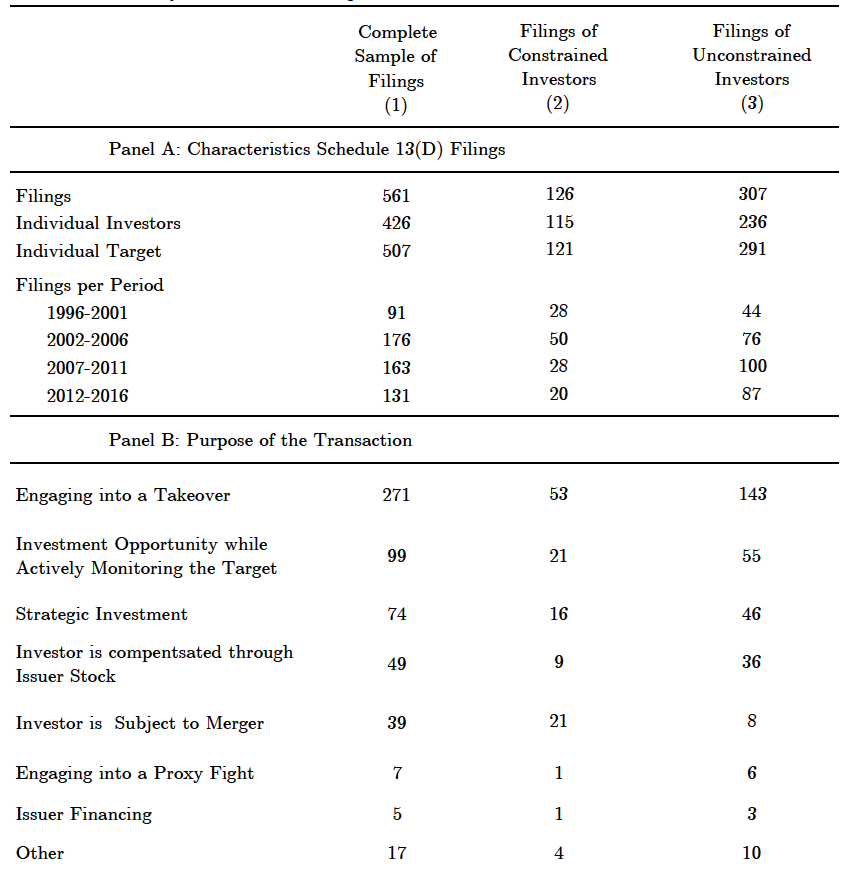
\includegraphics{descriptive1final}
	\end{adjustbox}\par\medskip
\end{table}
\begin{table}[!htbp]
	\centering
	\begin{adjustbox}{width=\textwidth}
		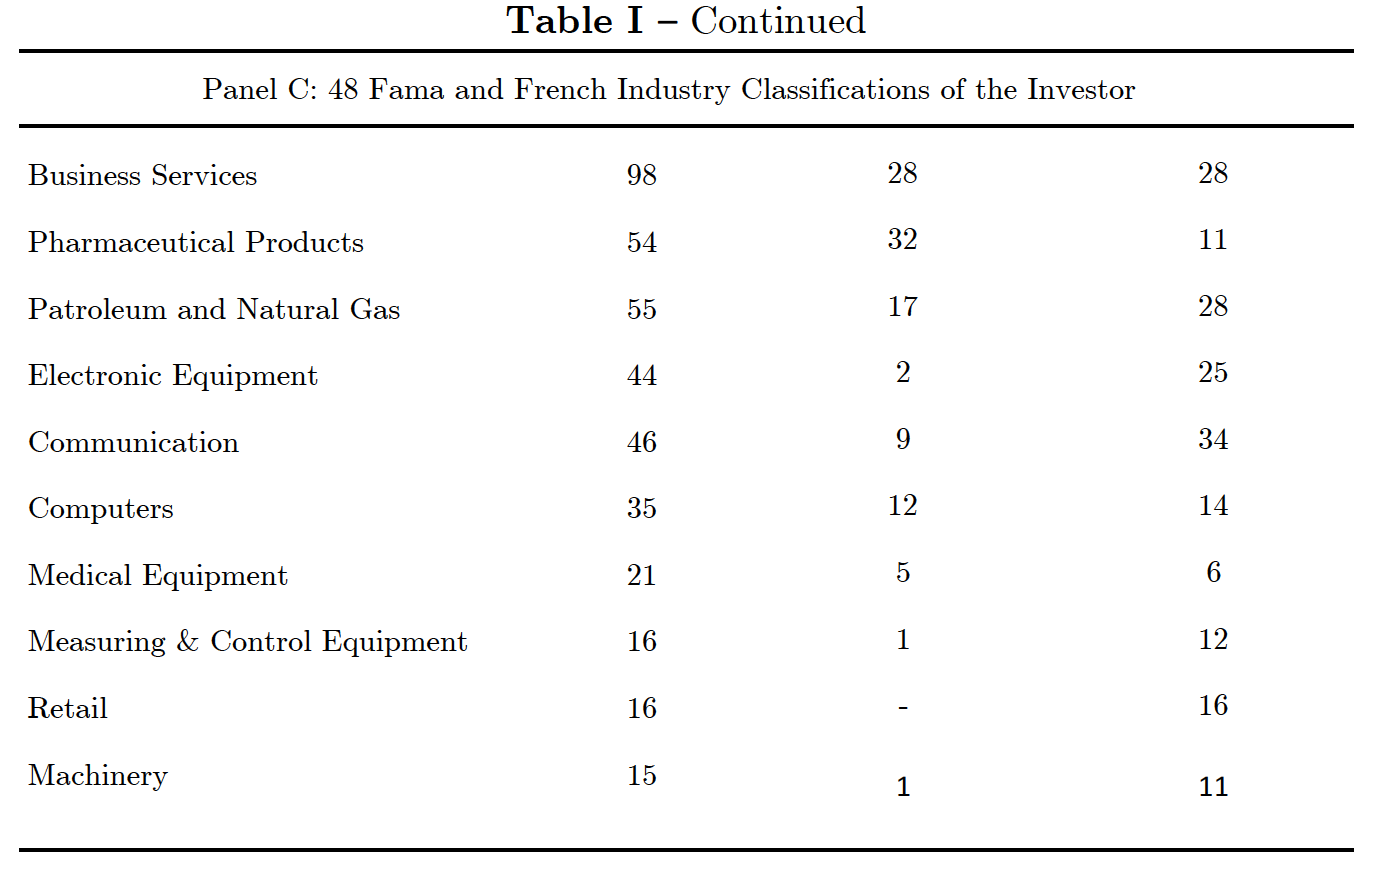
\includegraphics{descriptive2final}
	\end{adjustbox}
\end{table}
Panel B lists the extracted "Purpose of Transaction", which represents item 4 in Schedule 13(D) filings. The purpose is only explicitly stated if it occurs in at least five filings. Furthermore, the two purposes \emph{Engaging into a Takeover} and \emph{Strategic Investment} group several purposes by common characteristics. Following \citet[p.1]{Betton2008}, filings disclosed with the purpose of a merger agreement, tender offer or hostile bid are grouped under the purpose \emph{Engaging into a Takeover} and filings disclosed due to alliance agreements, license agreements, strategic acquisitions and joint ventures are grouped under the purpose \emph{Strategic Investment}. A detailed description on how the filings were categorized can be found in Appendix B.\par
Close to half of the investments were made while engaging into a takeover process and only 53 of these 271 filings were disclosed by constrained investors. On the other hand, more than half of the filings in which the investor was subject to a merger were disclosed by constrained investors -- the securities underlying the Schedule 13(D) were acquired to distribute them to own shareholders at the execution of the merger. In this scenario, the investor-target relationship is switched.
With 99 filings, the second most reported purpose was essentially to invest in the target. The target is considered to be a good investment opportunity, frequently undervalued and the investing corporation aims actively monitor and interact with it. The main idea is these filings do not directly imply future collaboration but give room for speculations.
Following actively held investments, strategic investments are the third most common purposes due to which filings were disclosed. Different to the former, they are based on the premise of future collaboration between investor and target and thus denote a likely value improvement for the target. Potentially of high interest, they represent around one quarter of filings. Although only 5 filings explicitly note direct financing as the purpose of transaction, 49 disclose the filing because they were compensated with issuer stock. Compensation can be a form of payment for cash-poor corporations and hence could also be classified as financing of the issuer. This is in line with the findings of \citet[p.2792]{Allen2000} and \citet[p.78]{Liao2014} who suggest one driver of minority acquisitions is the target's financing. Lastly, there are only 7 filings in which the investor announced a proxy fight with the target's management. In general, these presented transaction purposes are in line with the research findings on why corporation would actively hold equity ownership, namely in the process of takeover discussions, while building strategic alliances, for direct issuer financing or overcoming informational barriers.\par
Turning to Panel C, the major industries in which the investors operate according to their Fama \& French's 48 industry classification code are presented.\footnote{For simplicity, the SIC-Industry codes are not shown next to the Fama \& French industry classifications as these industries are compiled by several 3-digit SIC industries.} Shown are only industries, which are represented by at least 15 investors. For the complete sample, 42 out of the maximum 48 industries are represented. As mentioned previously, the sample is reduced by excluding the financial trading industry. The highest industry representation is in business services with 98 filings, followed by the industries of pharmaceutical products, petroleum and natural gas and electronic equipment. For the business industry, equally 28 are investors constrained and unconstrained. Looking at pharmaceutical products, there are more constrained than unconstrained investors and this proportion is also present in the computer industry. This could mean that especially in industries in which property rights become blurry and contracting is complicated hence information asymmetry is large, financially constrained firms have a higher representation \citep[p.4]{Liao2014}.

\subsection{Identifying the Investors prior to their Schedule 13(D) Filing}

\noindent After being familiar with general characteristics of the sample's filings, this section focuses on identifying the corporations prior to their Schedule 13(D) filing. What type of corporation makes activist investments and what are the characteristics of firms identified to be financially constrained? Do all these measures overall identify similar investors?\par
Following, Table II introduces financial characteristics of each measure's sub-samples.\footnote{Note that investors are classified into three groups based on the tertile values of the financial constraint indices but only the top and bottom groups are presented. There exists a "gray zone" in which investors are not directly classified.} By the virtue of each measure, the two samples do not necessarily have to add up to the total number of filings. Hence for the WW-Index, the two sub-samples consist out of 307 and 107 investors. By grouping the investors according to their dividend pay out ratio, 184 investors are identified to be financially constrained and 310 as not. The HP-Index identifies only 78 constrained investors in the initial sample and only for the rating measure do the two groups include all investors with 296 having a credit rating and 265 missing one. Lastly, the composite measure classifies 186 corporations to be financially constrained and 193 to be unconstrained.\par
For each sample, Table II reports the mean [median] of several key financials. For the complete sample, standard deviation and both, lowest and highest value are shown additionally. Column (1) and (2) present financials of the two sub-samples identified by each measure, where financially constrained investors are in Column (1) and unconstrained investors in Column (2). Column (3) shows the $t$-statistic and $Z$-statistic for differences between financially constrained and unconstrained investor's means and medians. For all following tests, the $t$-statistics are for differences in means, assuming unequal variances between the two samples. The null hypothesis to be tested is that the population means from the sample of constrained and unconstrained investors are equal $H_{0}: \mu_{1}=\mu_{2}$. The two-sided alternative hypothesis reads $H_{a}: \mu_{1}\neq\mu_{2}$, thus both means are unequal and there exists a difference. In addition to the parametric $t$-statistic, the non-parametric Wilcoxon Mann-Whitney $Z$-statistic tests, similar to \citet[p.201]{Klein2009}, whether the samples of constrained and unconstrained investors are from populations with the same distributions. It can also be called a test of differences in the medians, if the two sample distributions have the same shape. Specifically, the Mann-Whitney test is conducted by using the command -ranksum- based on \citet[p.59]{Mann1947}. All reported data correspond to the investor's fiscal year which is closest to the filing date and the reported values are winsorized at the 1\% and 99\% levels so that extreme values are replaced by the respective percentiles. This enables a presentation of more meaningful mean statistics \citep[p.203]{Klein2009}.   
\begin{table}[!htbp]
	\centering
	\captionsetup{textformat=empty,labelformat=blank}
	\caption{Characteristics of Investors prior to their Schedule 13(D) Filing}
	\textbf{Table II}\par\medskip
	\large\textbf{Characteristics of Investors prior to their Schedule 13(D) Filing}\par\medskip
	\justifying
	\footnotesize\noindent\setstretch{1.2}This table summarizes characteristics of the investors for the complete sample, and the sub-samples of each measure of investor's financial constraints (Columns 1 and 2). For the complete sample, standard deviation and minimum and maximum value of the variables are shown. For each variable, the mean [median] is reported. All data are winsorized at the 1\% and 99\% levels. Column (3) of each measure shows the t-statistic [Z-statistic] testing for differences between financially constrained and unconstrained investors means [medians]. All accounting data are from the end of the fiscal year closest to the reported Schedule 13(D) filing date. Panel A presents measures of the investor's profitability, Panel B displays  measures of cash balances and debt and Panel C gives information on the investor's size and Investment. See Appendix A for variable definitions. ***significant at the 0.01\% level; **significant at the 0.05\% level; * significant at the 0.10\% level.\par\medskip
	\centering													
	\begin{adjustbox}{width=\textwidth}
		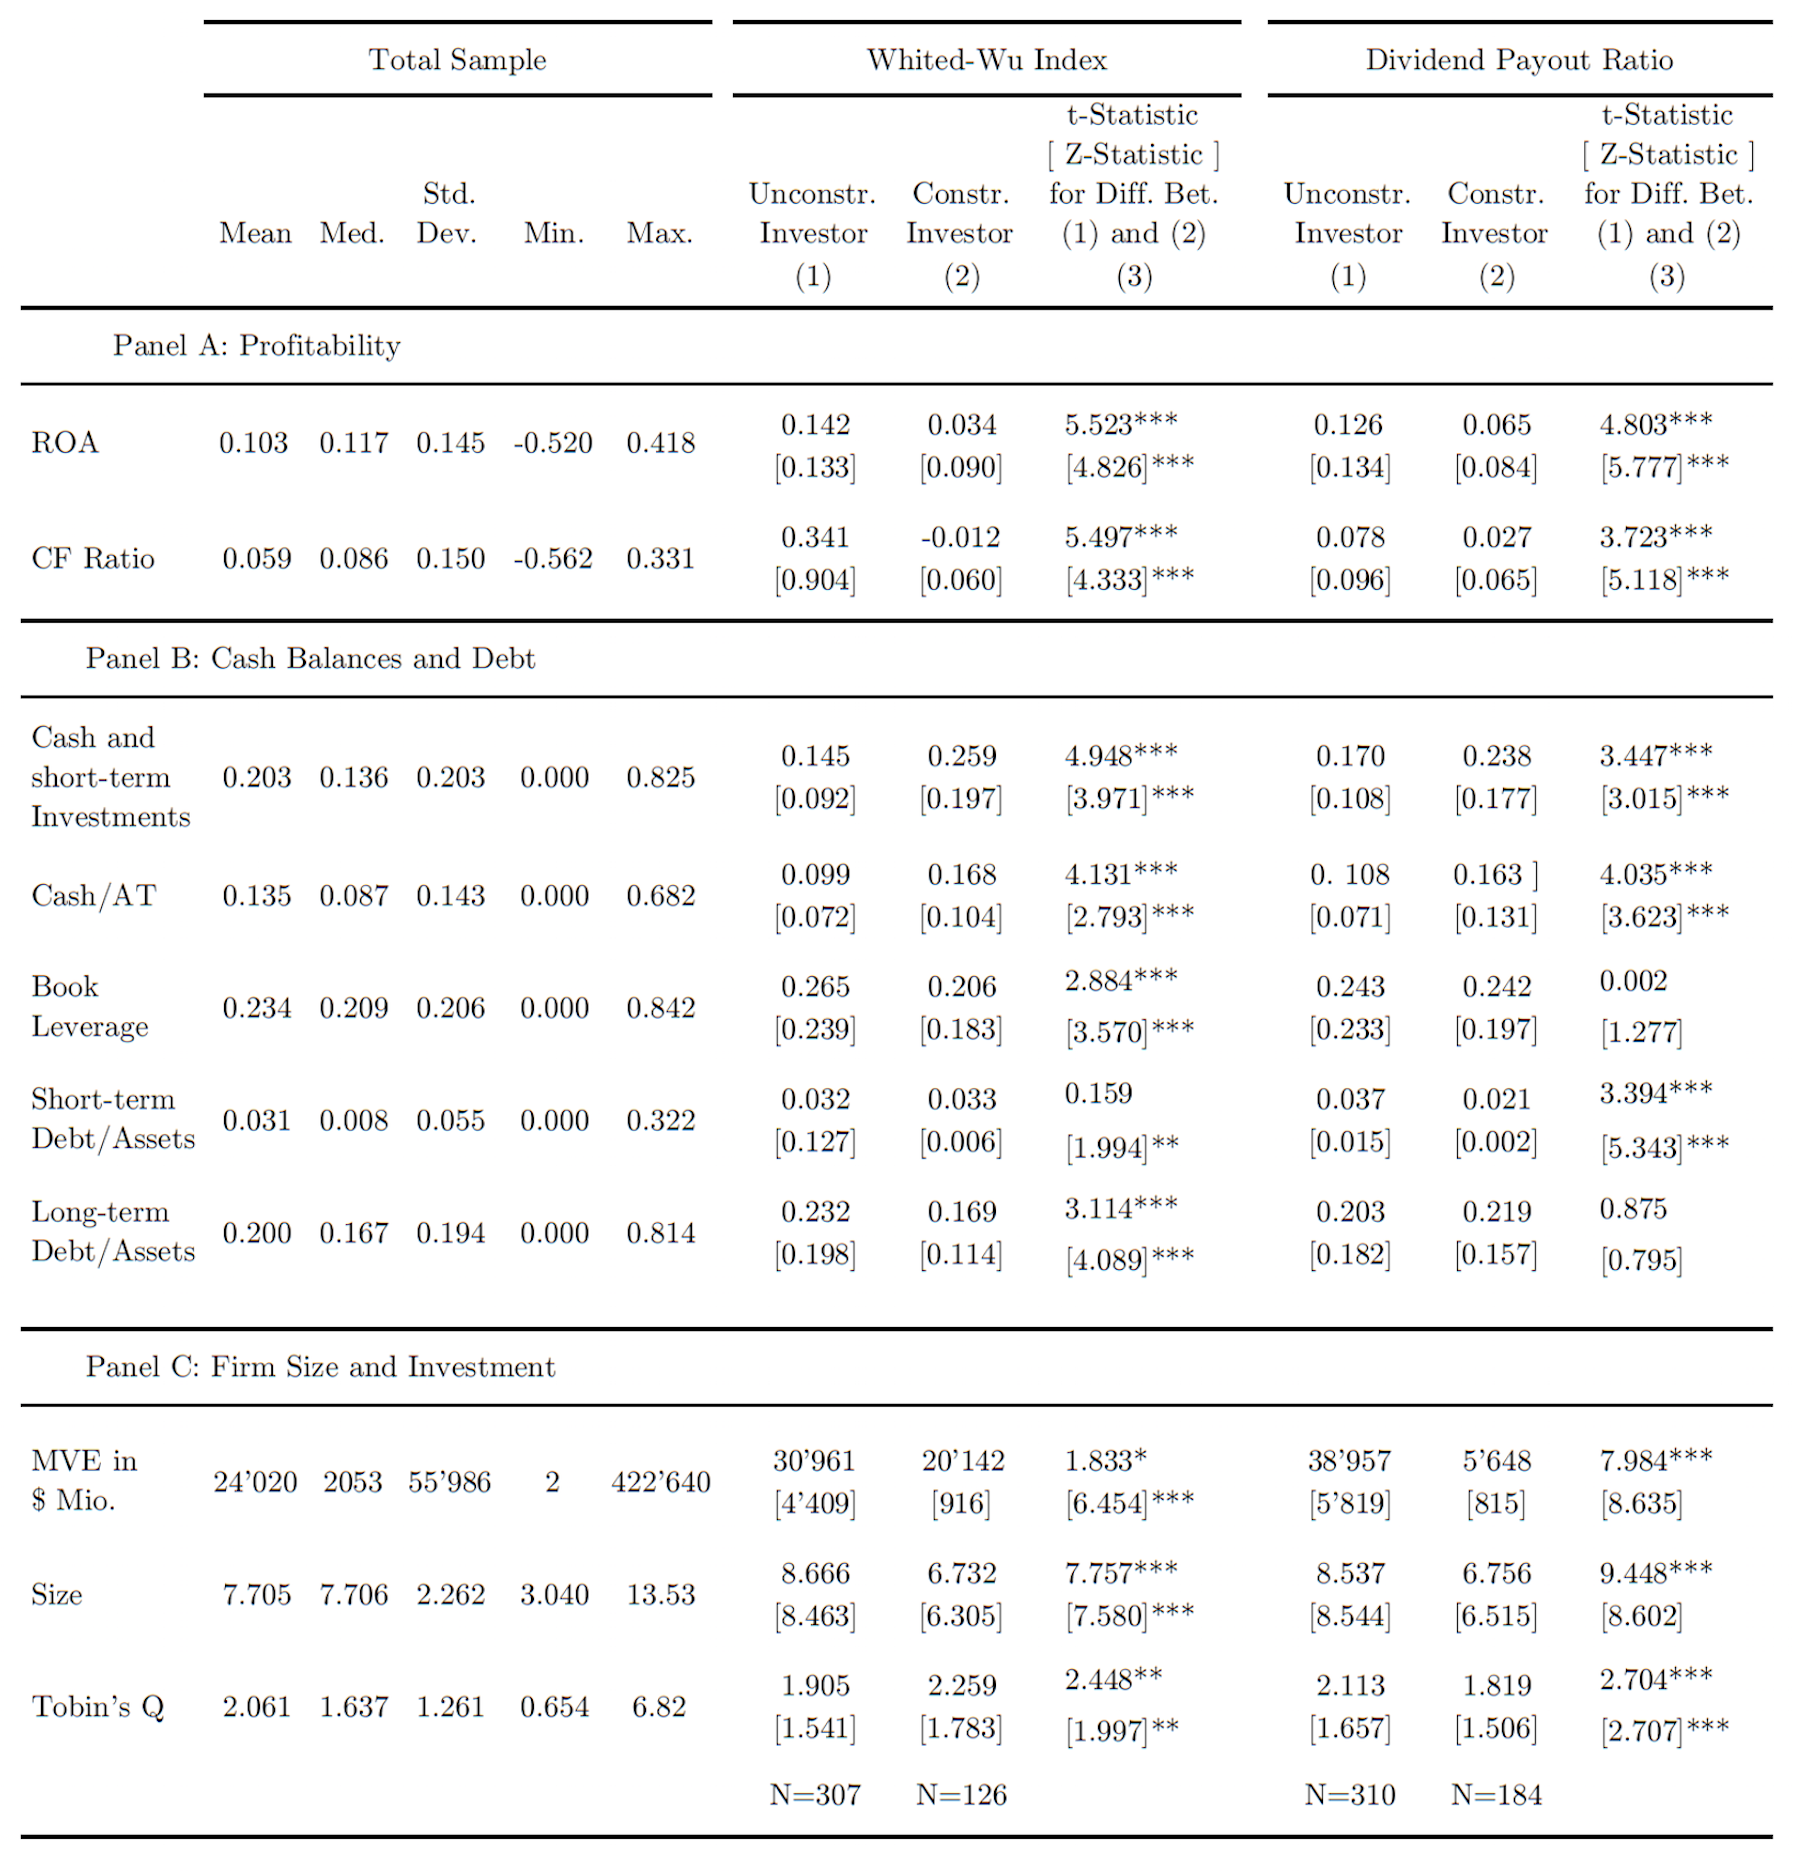
\includegraphics{Summary1_montag_copy}
	\end{adjustbox}\par\medskip
\end{table}
\begin{table}[!htb]
	\centering
	\begin{adjustbox}{width=\textwidth}
		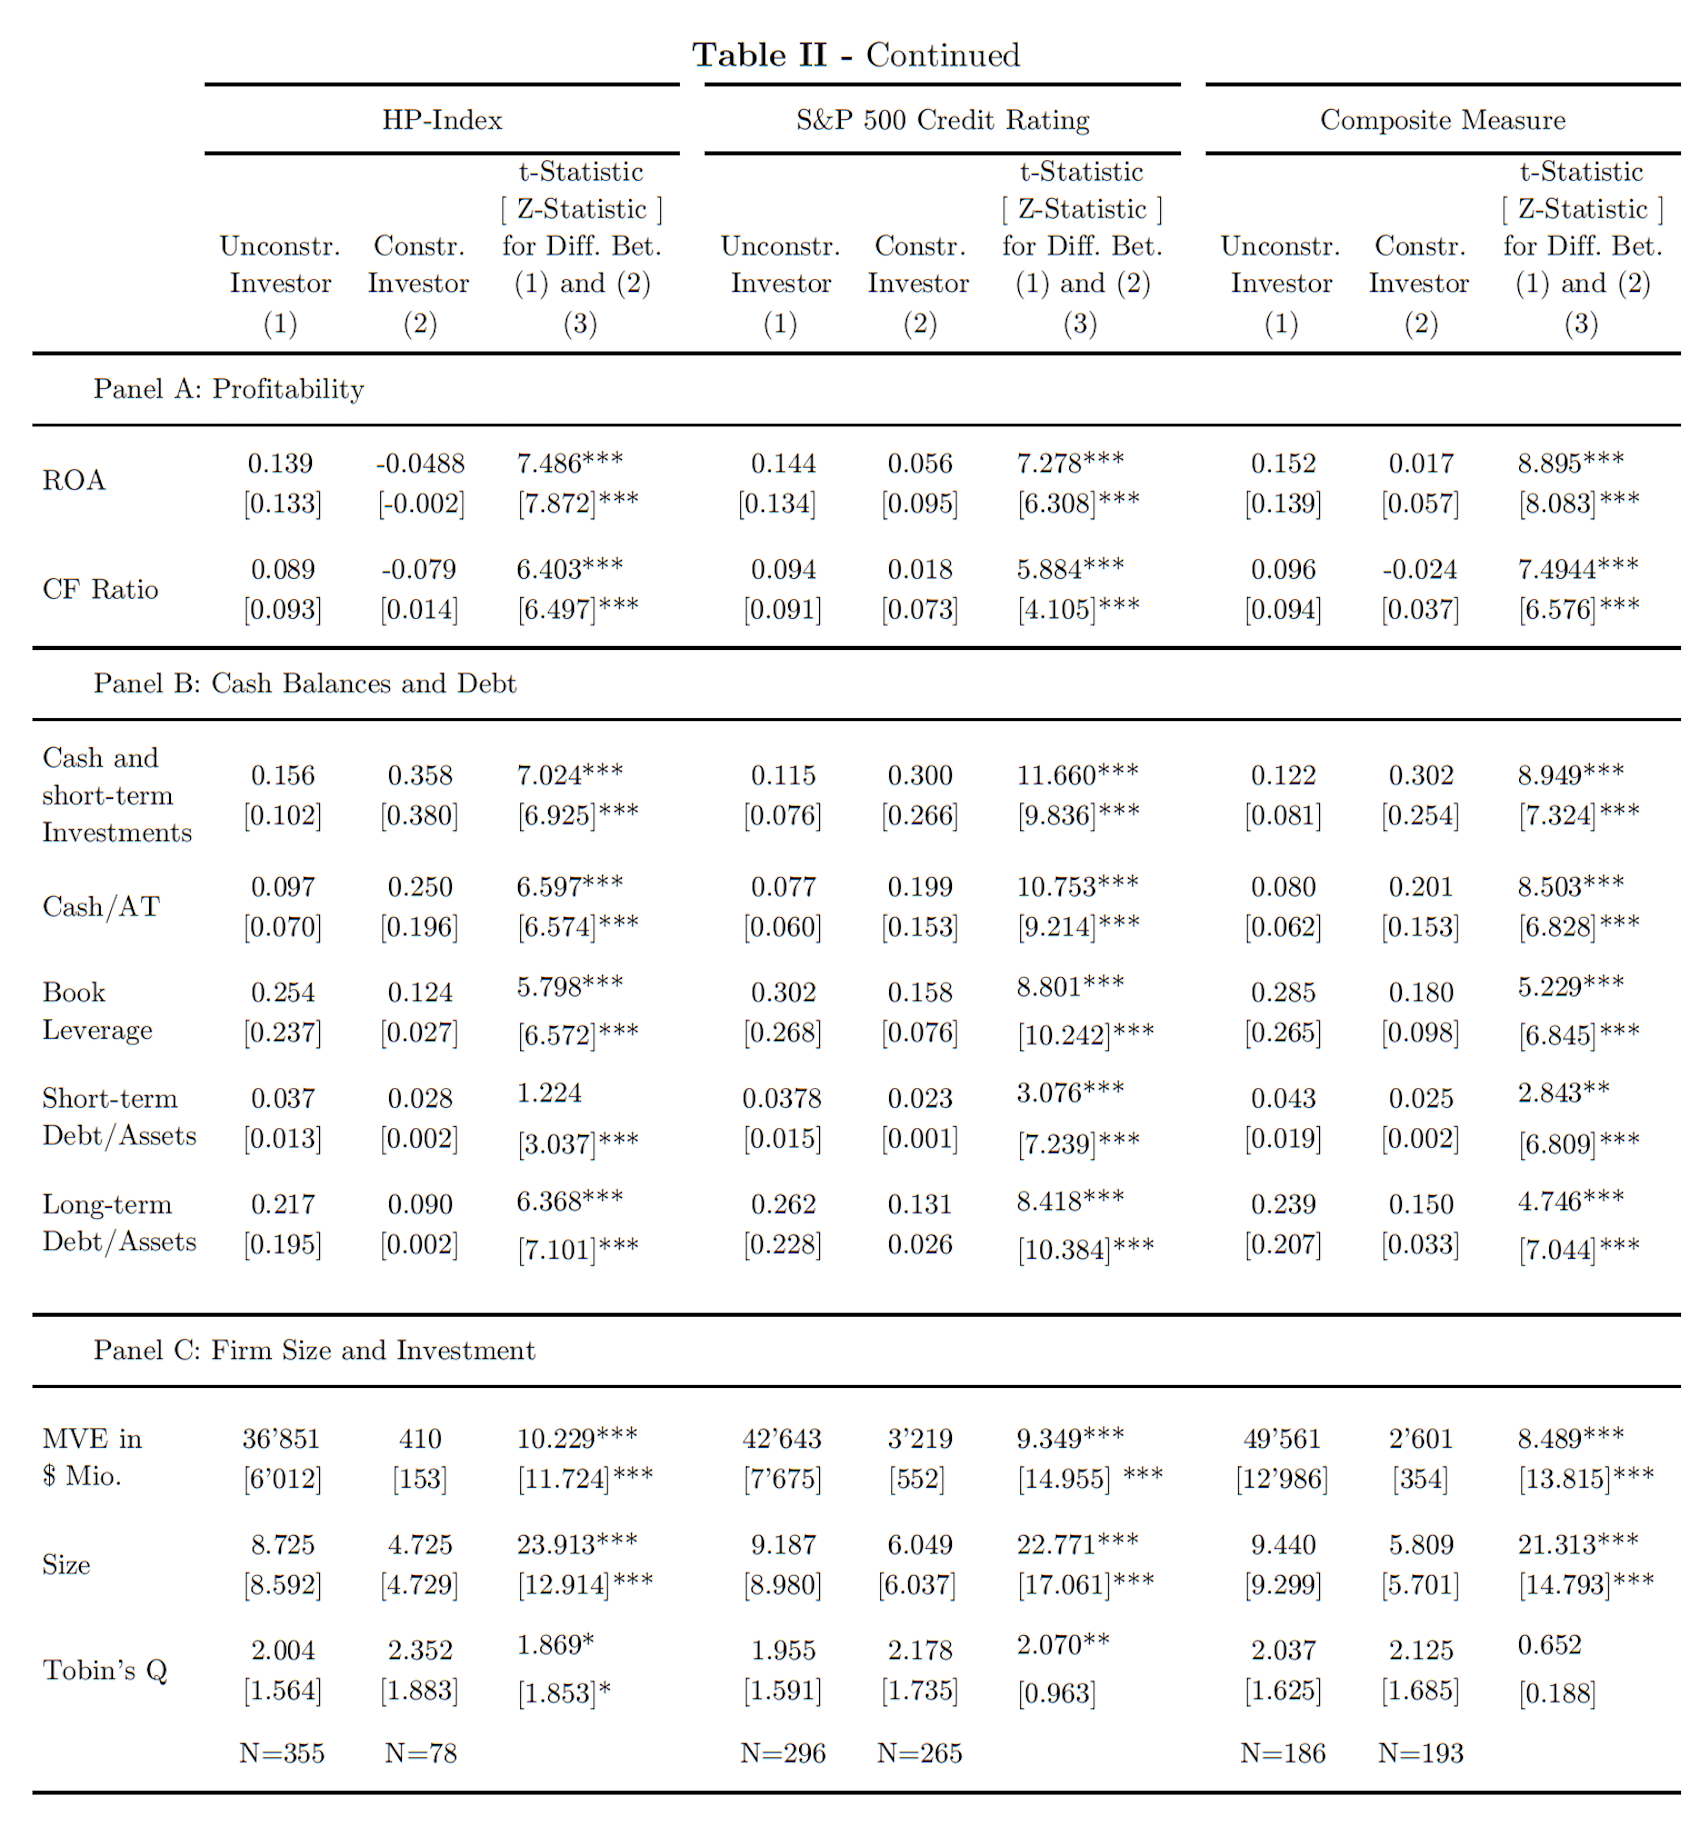
\includegraphics{Summary2_montag_copy}
	\end{adjustbox}
\end{table}
Moreover, characteristics for the WW-, HP- and Dividend Payout indices have explanatory power beyond the sample, as these investors are identified according to their comparative values across the entire Compustat database. Hence, a loose comparison to samples of other studies is possible. For further simplicity, the notion of "financially constrained" is used independently of the measure initially used for identification.\par
Panel A reports two ratios on profitability -- return on assets (ROA), defined as earnings before interest and taxes (EBITDA) to total assets and the ratio of cash flow from operations to total assets. On average, the sample's corporations have positive returns and a 0.059 cash flow ratio. Across all measures, financially constrained investors have a ROA which is significantly lower when compared to their counter-samples. Turning to the HP-Index, financially constrained investors even have a negative ROA in the fiscal year prior to the Schedule 13(D) filing. Furthermore, investors in this group also have a negative cash flow (same for the Whited-Wu index and the composite measure) and again, the difference between constrained and unconstrained investors is apparent and significant at the 1\% level across all measures. This implies that in general, constrained investors are less profitable \citep[p.544]{Whited2006}.\par
Panel B reports ratios on cash balances and debt. Constrained firms have considerably larger amounts of cash reserves (both cash and short-term investments) reflecting their dependency on internal funds when it comes to investments \citep[p.142]{Fazzari1988}. The difference in means is significant at the 1\% level across all measures and the largest for firms grouped by the HP-index. Unsurprisingly, book leverage, defined as long-term debt plus current debt to total assets \citep[p.1440]{MacKay2005} is higher for firms considered to be financially unconstrained, as financially constrained firms face the issue of restricted access to external finance. Significance in differences is given for all measures, except for the dividend payout ratio where the leverage levels are close to equal. Similar, the differences in the ratio of short-term debt to total assets are small but significant for firms grouped by their dividend payout ratio and credit rating. The sub-samples characteristics are similar to those presented in \citet[p.544]{Whited2006} and \citet[p.1917]{hadlock2010}, thereby suggesting a successful implementation of the measures on the sample of Schedule 13(D) filings.\par
Facing Panel C, information on firm size and investment is presented. The market value of equity is defined as the closing price at the end of the fiscal year times the number of shares outstanding. Through all measures, financially constrained firms have a lower market value of equity when compared to their counter samples. Except for the Whited-Wu index, the difference is significant at the 1\% level. The largest difference is among the two samples classified by the HP-Index. This however is unsurprising, as it only includes the two variables size and age with size playing a determining role. Similar differences are apparent in the variable size, defined as the natural logarithm of total assets. In conclusion, this suggests the investor's size is a determinant across all measures for firms identified to be financially constrained supporting the findings that size is an indicator of constraints. Lastly, Panel C also presents the investors investment opportunity in the form of Tobin's Q \citep[p.1441]{MacKay2005}, which is measured according to \citet[p.1]{Khatami2014}. Constrained firms have a higher Tobin's Q which may be evidence of their unexploited investment opportunities \citep[p.539]{Whited2006}.\par
To conclude, firms identified to be constrained in the sample of corporate activist investors are less profitable, hoard more cash and have smaller leverage compared to unconstrained firms. They are usually smaller in size and have more unexploited investment opportunities. Across all measures, the financial characteristics of financially constrained and unconstrained corporations tend to move in the same direction and show similarities to those of other studies (see \citet[p.544]{Whited2006} and \citet[p.1917]{hadlock2010})

\section{Market Response to Schedule 13(D) Filings -- Abnormal Stock Returns}
% Intention
\noindent In analyzing whether the financial condition of the activist corporate investor matters, abnormal share price reactions around the filing date identify the effect the 13(D) filing has on the target's stock, likewise the market's perception of value improvement, after accounting for general market movements.\par
The set up of the event study performed for this purpose is as follows: The time line consists successively of the estimation window, in which parameter estimates are obtained, the event window for which the abnormal returns are computed and the post event window. 
The filing date, as reported by the SEC and reported on Edgar is set as the event day. For simplicity, the event window [x,y] is determined relative to the event day 0 with x days before and y days after the filing date. Abnormal returns are computed for various event windows. For that reason, the estimation window is set 120 days prior to the largest event window. With the largest event window starting 30 days before the event day, the estimation window begins 150 days prior to the actual event day.\par
The abnormal return $AR_{i,t}$ for the target's security $i$ at day $t$ is defined as the difference between the actual (observed) return $R_{i,t}$ and the expected return $E(R_{i,t}|X{t})$ given the absence of the event \citep[p.15]{MacKinlay1997}:
	\begin{equation}\label{eq:1}
		AR_{i,t}=R_{i,t}-E(R_{i,t}|X_{t})
	\end{equation}
The expected return $E(R_{i,t}|X{t})$ is the result of an estimation based on the market model, in which the value-weighted NYSE/Amex/Nasdaq index from CRSP proxies for the market return $R_{M,t}$ and likewise is the independent variable \citep[p.18]{MacKinlay1997}.
	\footnote{For the expected return the market model assumes a constant and linear relation between the observed returns $R_{i,t}$ and the return of a market index $R_{m,t}$ \citep[p.18]{MacKinlay1997}. The parameters are estimated by ordinary least squares regressions based on estimation-window observations of stock returns.}
This yields the abnormal return $AR_{i,t}$
	\begin{equation}\label{eq:2}
		AR_{i,t}=R_{i,t}-(\hat{\alpha_{i}}+\hat{\beta_{i}}R_{M,t})
	\end{equation}
where $R_{i,t}$ is the actual return of security $i$ at day $t$ and $\hat{\alpha_{i}}+\hat{\beta_{i}}R_{M,t}$ are the ordinary least squared regression results from regressing the actual return $R_{i,t}$ on the market return $R_{M,t}$. To accommodate for a multiple period event window and to draw overall inferences of the Schedule 13(D) filings \citep[p.21]{MacKinlay1997}, the abnormal returns $AR_{i,t}$ for target $i$ are aggregated over the event window $(\tau_1,\tau_2)$.\par
For robustness, two different methods in aggregation over time are used. The cumulative abnormal return $CAR_{i,(\tau_1,\tau_2)}$ and the abnormal buy-and-hold return $BHAR_{i,(\tau_1,\tau_2)}$.\\
The cumulative abnormal return $CAR_{i,(\tau_1,\tau_2)}$ for security $i$ in event window $(\tau_1,\tau_2)$, is the sum of the abnormal returns $AR_{i,t}$ from equation \eqref{eq:2}.
	\begin{equation}
		CAR_{i,(\tau_1,\tau_2)}=\sum_{t=1}^{T}AR_{i,t}
	\end{equation}
The second method of aggregation over time is the abnormal buy-and-hold return $BHAR_{i,(\tau_1,\tau_2)}$. It is independent from the results of equation \eqref{eq:2} and no estimation window is required. 
The abnormal buy-and-hold returns $BHAR_{i,(\tau_1,\tau_2)}$ are the difference between the realized (observed) buy-and-hold returns and the normal buy-and-hold returns $R(R_{i,t}|X_{t})$.
In contrast to the cumulative abnormal return, the buy-and-hold return mimics the investment strategy of investors that buy the stock and hold it for a longer period of time. In this sense, the actual (normal) buy-and-hold return on day $t$ is the return on day $t$ times its lagged return on day $t_{-1}$ which in turn is the result of a multiplication with its lagged return $t_{-2}$. This means that for the target's security $i$ in the event window $(\tau_1,\tau_2)$ the abnormal buy-and-hold return $BHAR_{i,(\tau_1,\tau_2)}$ is
\begin{equation}
	BHAR_{i,(\tau_1,\tau_2)}=\prod_{t=\tau_1}^{\tau_2}(1+R_{i,t})-\prod_{t=\tau_1}^{\tau_2}(E(R_{i,t}|X_{t})
\end{equation}
Analogous to the estimation of normal returns for equation \eqref{eq:2}, the value-weighted NYSE/Amex/ Nasdaq index return from CRSP is used to proxy for the normal buy-and-hold returns $E(R_{i,t}|X_{t})$ in the respective event windows $(\tau_1,\tau_2)$ \citep[p.25]{Brav2009}.

\subsection{Time Series of Abnormal Returns}

\noindent Figure 1 plots the time series of the aggregation of average abnormal returns for securities subject to all filings and subject to filings of constrained and unconstrained corporate investors (grouped by the WW-Index) over the window [-30,10]. This means, average abnormal returns are calculated by grouping targets based on characteristics of the investor. A first glance reveals that independent of the investor, all three lines evolve almost equally until day -10. In the following days, targets of financially constrained investors experience smaller abnormal returns, that is their aggregation continues to proceed below the other two. Considering the fact they peak at around 8\%, targets of unconstrained investors experience cumulative abnormal returns considerably higher with close to 20\%. In-between, abnormal returns for the complete sample of targets aggregate to approximately 15\% during the 41-day window. This is approximately 5\% more compared to the 10\% reported in \citet[p.1563]{Collin-Dufresne2015}. 
Figure 1 indicates that abnormal returns in the [-30,10] window for targets of financially constrained investors differ in magnitude and thus presents first evidence that financial constraints of corporate activist investors could matter.
\begin{figure}[!htb]
	\centering
	\captionsetup{textformat=empty,labelformat=blank}
	\caption{Time Series of Cumulative Abnormal Returns}
	\begin{adjustbox}{width=\textwidth}
		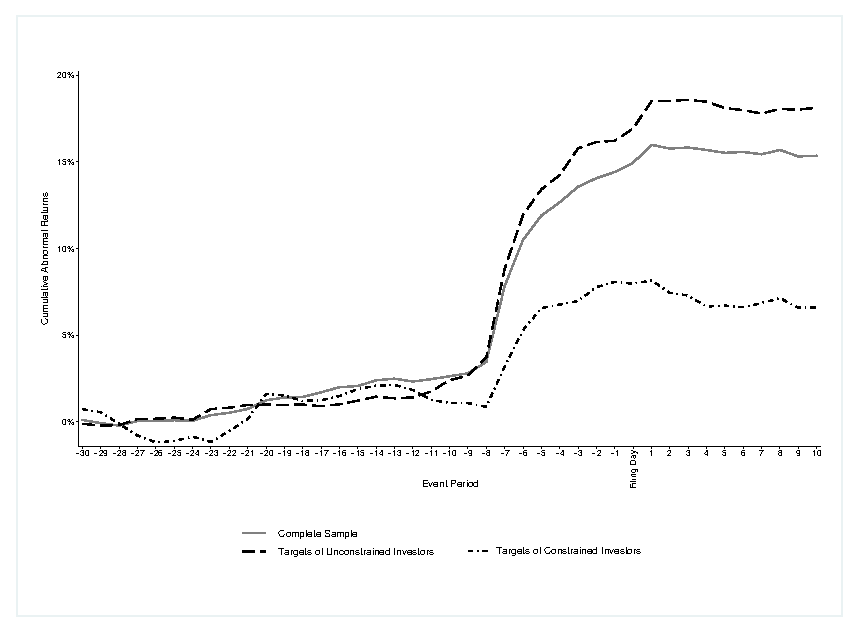
\includegraphics{WW-TimeS_copy.eps} \label{AR}
	\end{adjustbox}
	\justifying
	\noindent\footnotesize\setstretch{1.2}\textbf{Figure 1. Time Series of Cumulative Abnormal Returns.} The solid line plots the time series of average cumulative abnormal returns for all targets where the cumulative abnormal returns is the aggregation of abnormal returns up to each point in time using the market model with the value-weighted NYSE/AMEX/Nasdaq index from CRSP as the market return from 30 days prior to the filing date to 10 days afterwards. Equivalently, the dashed (dashed-dot) line plots the average cumulative abnormal returns for targets of financially unconstrained (constrained) investors. \par\medskip
\end{figure}
Furthermore, Figure 1 reveals that in all three cases, abnormal returns start to occur extensively in the [-11,-8] period, implying that valuable information -- in any form -- is available before the actual filing. Although the behavior is in line with that presented in \citet[p.1563]{Collin-Dufresne2015}, \citet[p.370]{Greenwood2009} and \citet[p.1756]{Brav2008}, possible explanations are the following: Stock market participants might knew about the pending stake before it was announced, for which \citet[p.2802]{Allen2000} choose their event window to be [-10,10]. This is equivalent to information leakage for which \citet[p.31]{Brigida2012} find evidence prior to the actual filing date. Furthermore, filings may not be reported until several days after the actual investment for which reason \citet[p.87]{Liao2014} also implements a longer event window. These possibilities are in line with general characteristics of Schedule 13(D) filings, as Section 13(d) grants the investor a 10-day window after passing the 5\% threshold for disclosing the filing and thereby allowing for the possibility of information leakage and delayed disclosure.\par
As it are the investor's own actions that potentially increase the value of the target firm, a potential increase in their trading activity could also explain the early upsurge. This approach is adopted from  \citet[p.1561]{Collin-Dufresne2015} who analyze the trading strategy of informed Schedule 13(D) filers. Firstly, they find that trading activity increases in the [-12,-9] period in which the reported event dates are clustered (date on which the 5\% threshold is passed). Secondly, they show that close to 1\% of outstanding shares are purchased on the event date, compared to only 0.10\% and 0.15\% on the days before and after the event date \citep[p.1561]{Collin-Dufresne2015}. Thirdly they note that the prices move up when Schedule 13(D) filers trade. By combining these three findings, an explanation could be that by their own trading at the event day, corporations drive up prices. This argument however is limited, as constrained firms experience small negative abnormal returns in this period. Summarizing these explanations, \citet[p.207]{Klein2009} start their event window at day -30 to allow for the 10-day 13(D) filing window, possible prior leakage of information and prefiling price pressure.\par
That is to say, these researchers have expanded their event-windows to overcome the difficulty of identifying the precise date on which the information reaches the market. This adjustment might create problems as the number of confounding events increases \citep[p.352]{mcwilliams1999}. For that reason, the sample of Schedule 13(D) filings was cross-referenced with a sample of activism filings provided by SharkRepellent. This however lead to only 40 matched campaigns occurring in the respective month of the target's Schedule 13(D) filing. For these 40 matches, the reported announcement date by SharkRepellent was either equal to or later than the reported filing date of the Schedule 13(D), thereby revealing no additional information.

\subsection{Event Windows and Financial Constraints}

\noindent For the aforementioned reason, Table III presents the mean [median] cumulative and buy-and-hold abnormal returns for the following four event windows: Event window 1 is [-10,3], to allow for the 10-day filing window, information leakage and accommodate subsequent press coverage. The second event window is [-10,-6] to detach the possible effect of information leakages and event-date trading. Analogous, the third event window [-5,3] aims to control for these two. This seems to be reasonable, as the aggregation of abnormal returns in Figure 1 slows down at around day -5, implying that information has been processed. The fourth event window is [-1,3] to accommodate for just the filing date and press coverage.
\begin{table}[!htbp]
	\centering
	\captionsetup{textformat=empty,labelformat=blank}
	\caption{Abnormal Stock Returns Surrounding the Schedule 13(D) Filing}
	\textbf{Table III}\par\medskip
	\large\textbf{Abnormal Stock Returns Surrounding the Schedule 13(D) Filing}\par\medskip
	\justifying
	\footnotesize\noindent\setstretch{1.2}This table presents the cumulative and buy-and-hold abnormal returns of the targets. The CAR is the aggregated abnormal return from the market model and the BHAR is the difference between the target's buy–and–hold return and the value–weighted NYSE/AMEX/Nasdaq index from CRSP. Mean [median] abnormal returns  are reported for the total sample of targets (Column 1) and  for targets of investors identified by the WW–Index (Column 2 and 3). Panel A--D present abnormal returns for several event windows. All data are winsorized at the 1\% and 99\% levels. *, ** and *** indicate statistical significance at the 10\%, 5\% and 1\% levels.\par\medskip
	\centering				
	\begin{adjustbox}{width=\textwidth}
		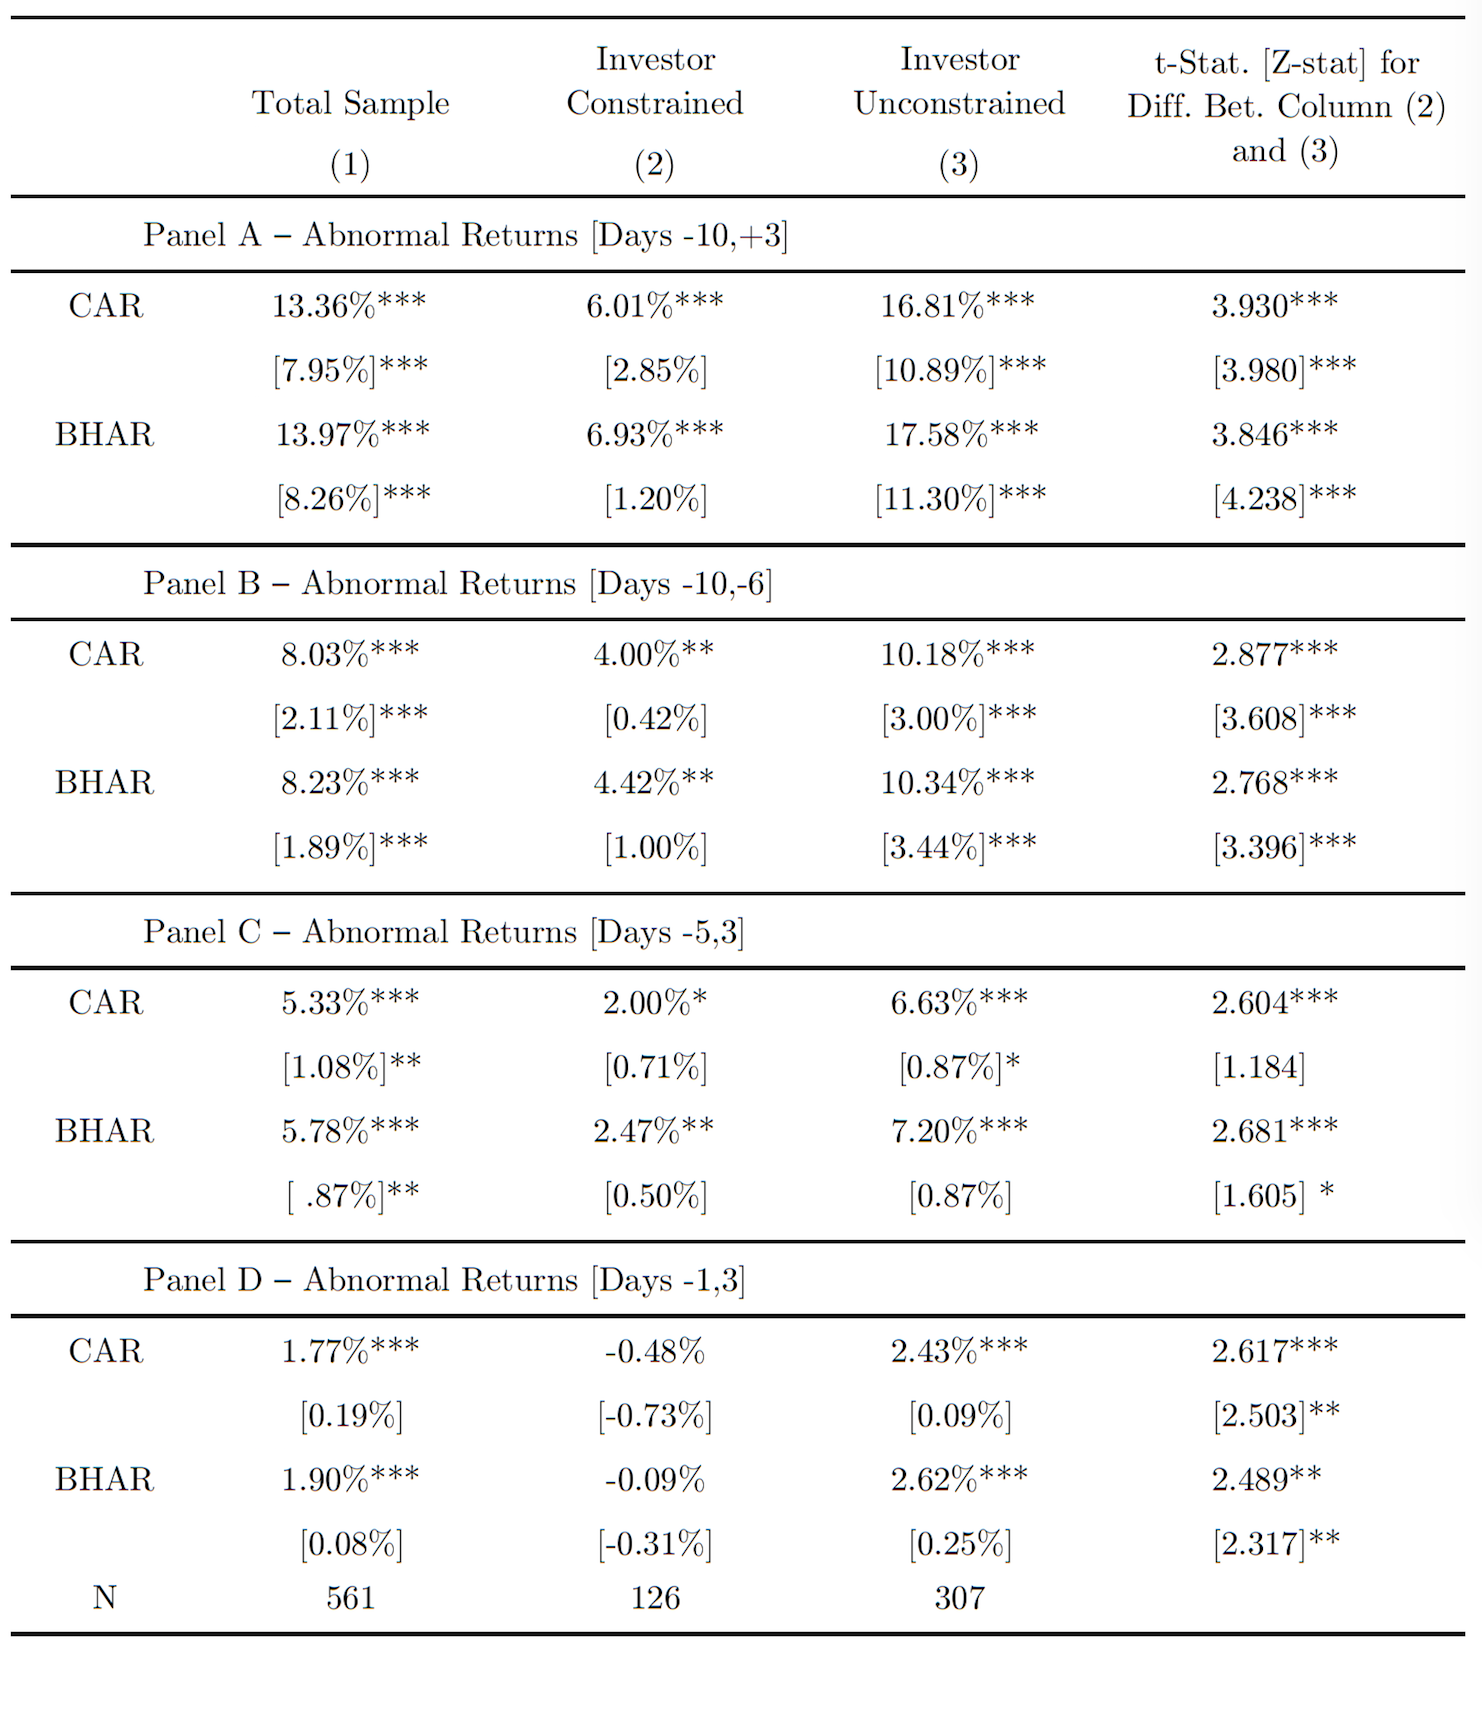
\includegraphics{Ar_window_montag_copy}
	\end{adjustbox}\par\medskip
\end{table} 
Column (1) presents the abnormal returns for all targets. Column (2) and (3) show the abnormal returns for targets dependent on their investor's financial condition. The investors are grouped by the Whited-Wu index and groups are equal to those presented in Table II, with 126 filings disclosed by constrained and 307 disclosed by unconstrained investors.\par
For the abnormal returns in columns (1), (2) and (3), significance levels are shown. The null hypothesis to be tested is that the mean day abnormal return is equal to zero, and thus concerns the average effect of an event on returns to shareholders. If the average abnormal returns are independent, identical distributed, and normal, the test statistic is distributed Student-$t$ under the null hypothesis \citep[p.7]{Brown1985}. As shown in \citet[p.11]{Brown1985}, the $t$-Statistic can be applied even under the assumption of non-normality and a sufficient adjustment for cross sectional dependence is the application of the market model for estimating abnormal returns \citep[p.22]{Brown1985}. Therefore, the statistical significance of the cumulative abnormal returns is given by a two-tailed $t$-test for which the alternative hypothesis is defined as: cumulative abnormal returns are different from zero. The statistical significance of the median is computed by a quantile regression of the abnormal returns where the p-value of the coefficient represents the statistical significance of the median \citep{Ucla}. Column (4) tests the difference in means [medians] of column (2) and (3). As in Section 3, the $t$-statistic represents the standard parametric test for difference in means and the $Z$-statistic is the non-parametric Mann-Whitney rank-sum test. All returns  presented in Table III are winsorized at the 1\% and 99\% level.\par
This extensive presentation of aggregated abnormal returns is done for three reasons. Firstly, to test the differences in abnormal returns over varying event windows and thereby accomodate for the time-effect. Secondly, to test whether the estimated abnormal returns are similar for the two methods of measurement and thirdly to test whether the investor's financial condition matters independently of time (across all event windows).\par
Panel A presents the abnormal returns for the largest event window [-10+3]. Both, cumulative and buy-and-hold abnormal returns are positive and strongly significant at the 1\% level with mean abnormal returns being 13.36\% and 13.97\% respectively. Consistent with Figure 1, targets of unconstrained investors have a mean CAR and BHAR of 16.81\%, around 10\% higher when compared to those of constrained investors. For both, CAR and BHAR, the difference in abnormal returns across the two groups is statistically significant at the 1\% level. This shows, the investor's financial condition does matter economically and statistically when comparing the two means. These findings are supported by differences of around 7\% in medians. Furthermore, the abnormal returns of around 13\% are different to those observed in \citet[p.208]{Klein2009} but support \citet[p.29]{Brigida2012} findings that abnormal returns are higher for non-financial corporations.\par
Turning to panel B, the largest runup happens in the [-10,-6] event window. Abnormal returns aggregate to around 8\%, making up more than 50\% of the total [-10,3] runup. These results are matching with \citet[p.32]{Brigida2012} who find that the target's runup is greatest during the event window [-10,-6]. Again, targets of weak investors only gain 4\% whereas those of unconstrained investors have abnormal returns up to 10.30\%. Furthermore, the difference in means is is significant at the 1\% level for both methods of estimation.\par
% was will ich hier eigentlich sagen!! 
In Panel C, abnormal returns for the event window [-5,3] are shown. Independent of the investor, all targets experience a mean CAR of 6.63\%, significant at the 1\% level. Here too, targets of unconstrained investors outperform those of weak investors with around 5\%, while being statistically significant at the 1\% level.\par
Turning to abnormal returns for the smallest event window [-1,3] in Panel D, targets on average gain 1.77\% which is significant at the 1\% level. Hence positive abnormal share price reactions at the announcement of the filing exists and are not only apparent for the previous days. Striking is that on average, targets of constrained investors now experience negative returns but statistically not different from zero. Furthermore, the difference of approximately 2\%  among the two samples is considerable, especially  when considering the short event window and the already low-level of abnormal returns.\par
Concluding, both buy-and-hold and cumulative abnormal returns show similar results with positive and significant share price increases in all event-windows surrounding the Schedule 13(D) filing date. Furthermore, the largest aggregation happens in the [-10,-6] event window but is not exceptionally high when compared to the overall runup. Most importantly however is the difference in average abnormal returns for targets of financially constrained and unconstrained investors. The difference is present, both on an economic and statistical level. When testing the differences in means, the difference is significant across all event windows, thus presenting further evidence that financial constraints matter, independent of the event-windows of aggregation.

\subsection{Purpose of Transaction and Financial Constraints}

\noindent So far it has been shown that independent from the event window, targets of financially unconstrained corporate investors gain on average significantly more, when compared to those of financially constrained investors. Attached thereto, this section aims to analyse whether this difference is existent both, across filings' different transaction purposes and for different measures of financial constraints.\par
For this reason, Table IV presents the mean [median] cumulative abnormal returns from the [-10,+3] event window for each each measure and further for different transaction purposes. In using the longer event-window, the analysis follows various studies, both on Schedule 13(D) filings and corporate equity announcements (see \citet[p.369]{Greenwood2009}; \citet[p.210]{Klein2009}; \citet[p.1758]{Brav2008}; \citet[p.87]{Liao2014}). The measures of financial constraints and among which the sample separation takes place are the Whited-Wu Index, the investor's dividend payout ratio, the HP-Index, the investor's S\&P's long-term issuer credit rating and lastly the composite measure. For comparison, Panel A shows the mean cumulative abnormal returns for the complete sample of targets whereas Panel B presents the mean cumulative abnormal returns dependent on the filing's purpose of transaction. Hence \emph{Engaging into a Takeover} involves merger agreements, tender offers and hostile bids and \emph{Strategic Investments} represents alliance agreements, license agreements, strategic acquisitions and joint ventures. \emph{Remaining Purposes} groups the abnormal returns for the remaining transaction purposes. This particular grouping is done to enable a better comparison to relevant other studies and to have larger sample sizes on which tests can be conducted. For each measure, Column (1) and (2) present mean [median] cumulative abnormal returns for the two sub-samples. Column (3) tests the difference between column (1) and (2) and displays the  $t$-statistic [$Z$-Statistics].\par
Turning to Panel A, average abnormal returns for all samples, without specifying the transaction purpose, are presented. Across all measures, targets of financially constrained investors have significantly lower abnormal returns in the [-10,3] event window. Starting with the samples formed by the Whited-Wu index, the difference for the mean CAR is 10\% and significant at the 1\% level. Targets of unconstrained investors gain 16.81\% and those of constrained only 6\%. Similar conclusions can be drawn when comparing the samples grouped by the investor's dividend payout ratio. Targets of constrained investors encounter abnormal returns of 9.79\% compared to 15.76\% for unconstrained investors. Again, the difference in means is significant at the 5\% level and comparing the sub-samples of the HP-index yields similar results -- targets of constrained investors experience abnormal returns of 9.18\%, those of financially unconstrained investors 16.2\% and the 7\% difference in means is significant but only at the 5\% level. On the other hand, the difference in market reactions to filings of investors with and without a credit rating is present but has no statistical significance. An explanation could be a possible upward bias in mean abnormal returns for the sample of constrained investors, as some of the least constrained corporations might lack a credit rating and are therefore mistakenly identified as financially constrained \citep[p.18]{heller2015}. Supporting above findings, the composite measure shows similar results. Targets of financially constrained investors gain around 10\% less in the [-10,3] window, which is significant at the 1\% level.\par
Across all measures is a difference in the mean cumulative abnormal returns visible and not only apparent when applying the Whited-Wu Index as in the previous section. The persistence across different measures of financial constraints further indicates that financial constraints could matter when the market assesses the value improvement for the target.\par
Facing Panel B, abnormal returns of targets are now additionally sorted by the filing's purpose of transaction. The purpose of engaging into a takeover generates the strongest market reaction with a mean CAR of 21.45\% for the 271 targets and cross all measures, targets of financially unconstrained investors have a CAR of roughly 25\% for the [-10,3] event window. \citet[p.112]{Khatami2014} have similar results for acquisition announcement returns when the acquirer is financially unconstrained with an 11-day CAR of 25\%. The difference in abnormal returns is the largest for the Whited-Wu index and the smallest for the investor's credit rating which is analogous to Panel A. For all measures, except the HP-index, the difference in mean CAR's is significant at least at the 5\% level. For targets of investors grouped by the HP-Index, the difference is significant only at the 10\% level which might be due to the low sample size of only 43 filings from constrained investors. Nonetheless, this univariate comparison reveals that investors' financial constraints might be especially important in the context of mergers and acquisitions \citep[p.112]{Khatami2014}.
\begin{table}[!htbp]
	\centering
	\captionsetup{textformat=empty,labelformat=blank}
	\caption{Abnormal Returns by Measures of Financial Constraints and Purpose of Transaction}
	\textbf{Table IV}\par\medskip
	\large\textbf{Abnormal Returns by Measures of Financial Constraints and Purpose of Transaction}\par\medskip
	\justifying
	\footnotesize\noindent\setstretch{1.2}This table shows cumulative abnormal returns aggregated over the window [-10,3] for the sub-samples of each measure of financial constraints. Mean [median] target abnormal returns of each measure are reported for the sample of financially constrained (Column 1) and unconstrained investors (Column 2). Column (3) presents the t-statistics [Z-statistics] for differences in means [medians] of Columns (1) and (2). Panel A shows the cumulative abnormal returns for the complete sample of targets whereas Panel B presents the cumulative abnormal returns for targets based on the purpose of transaction. The purposes are equal to those presented in Section 3. See Appendix A for Measure and Appendix B for Purpose definitions. All data are winsorized at the 1\% and 99\% levels. *, ** and *** indicate statistical significance at the 10\%, 5\% and 1\% levels.\par\medskip
	\centering				
	\begin{adjustbox}{width=\textwidth}
		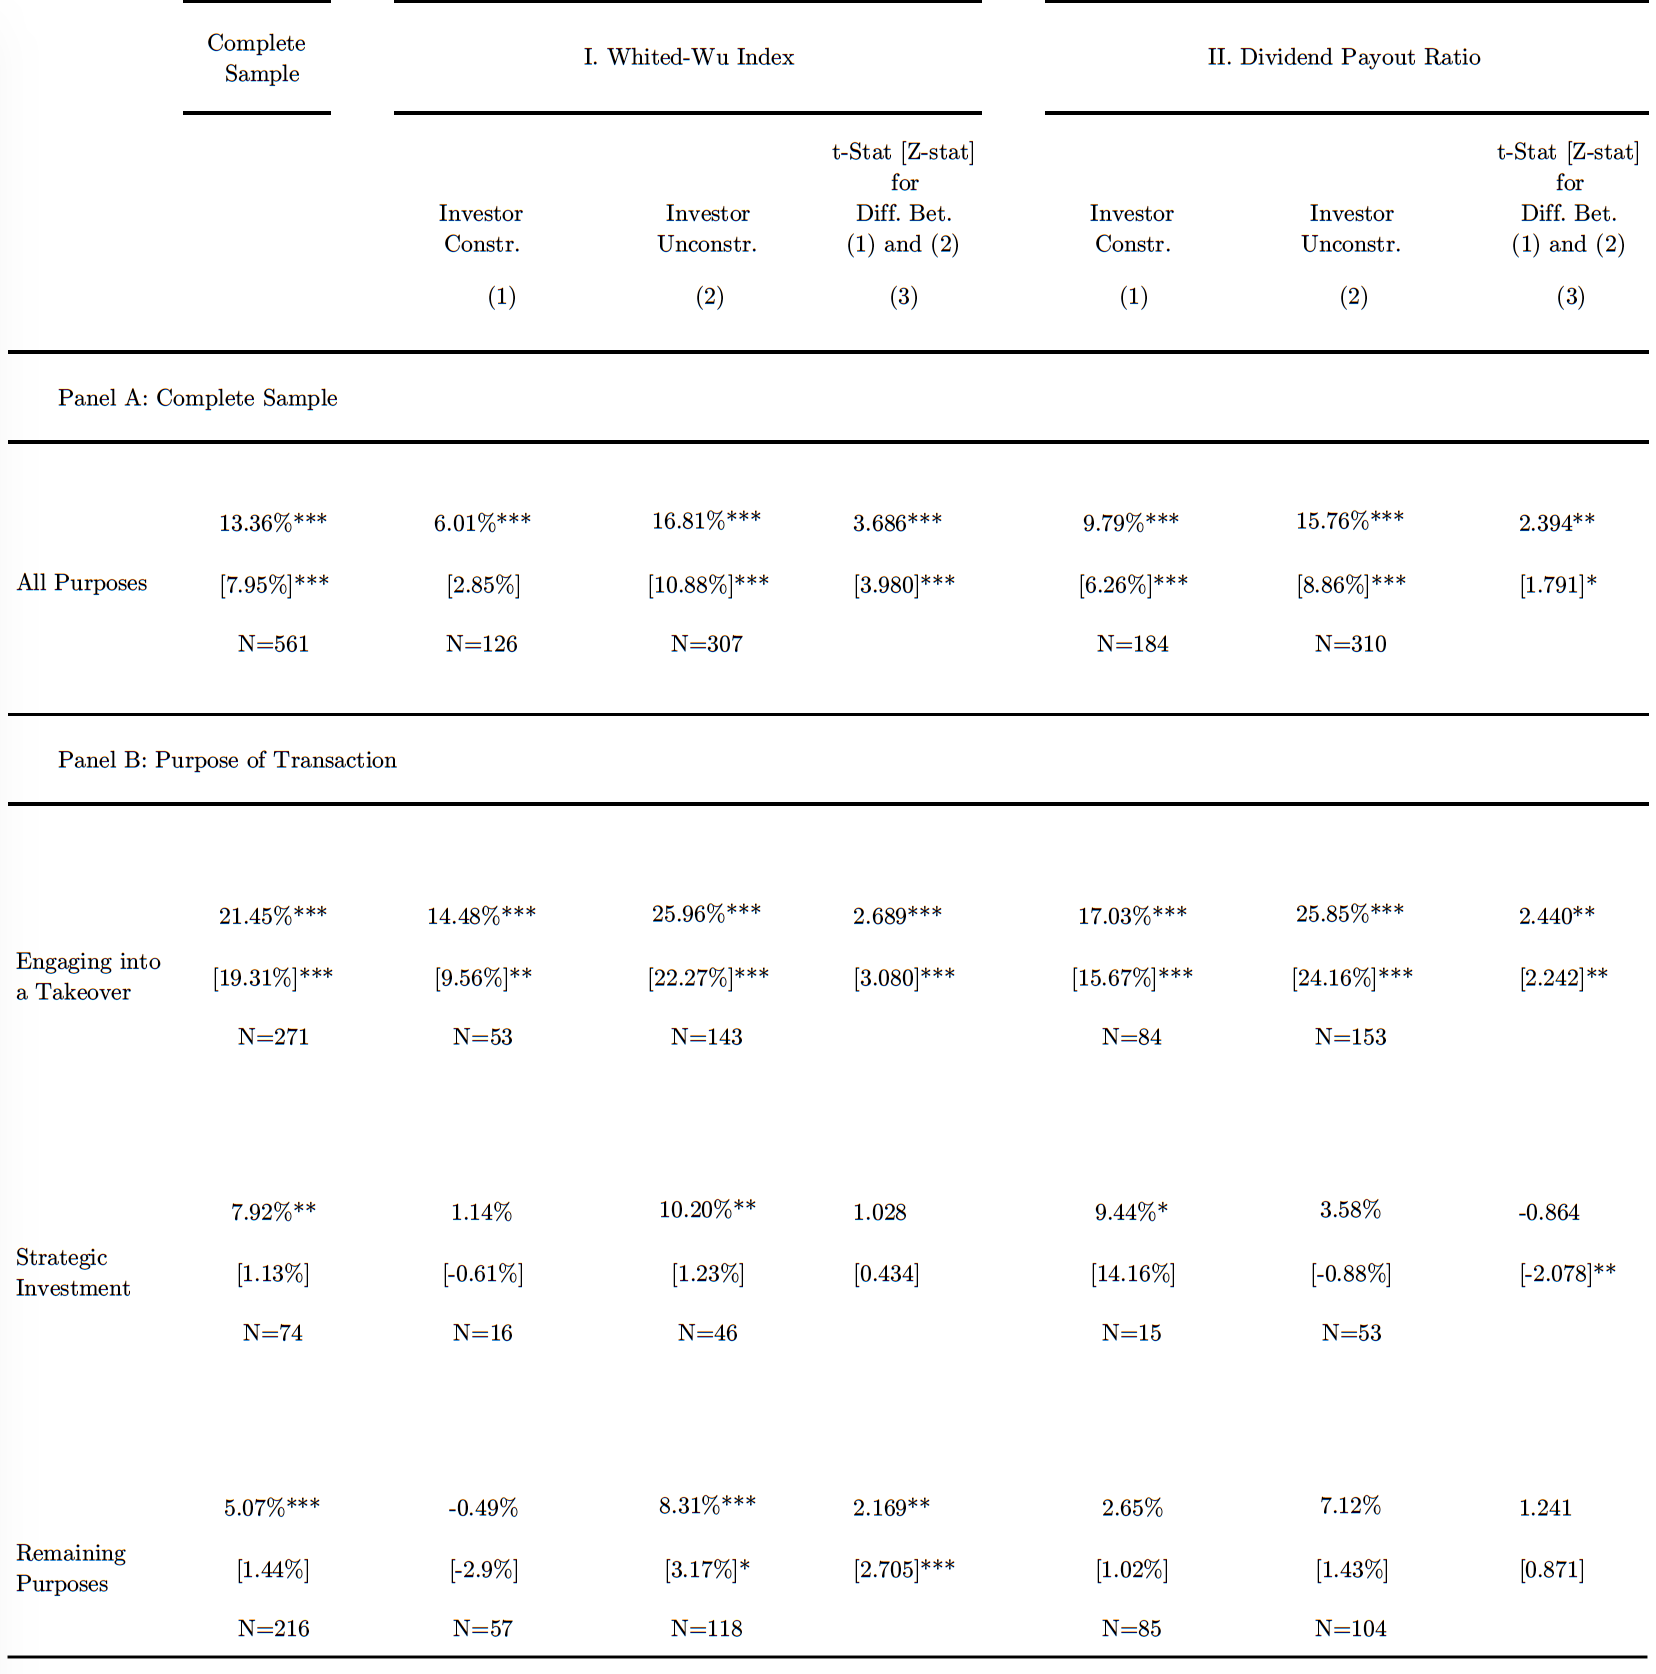
\includegraphics{Ar_measure1_montag_copy}
	\end{adjustbox}\par\medskip
\end{table}
\begin{table}[!htb]
	\centering
	\begin{adjustbox}{width=\textwidth}
		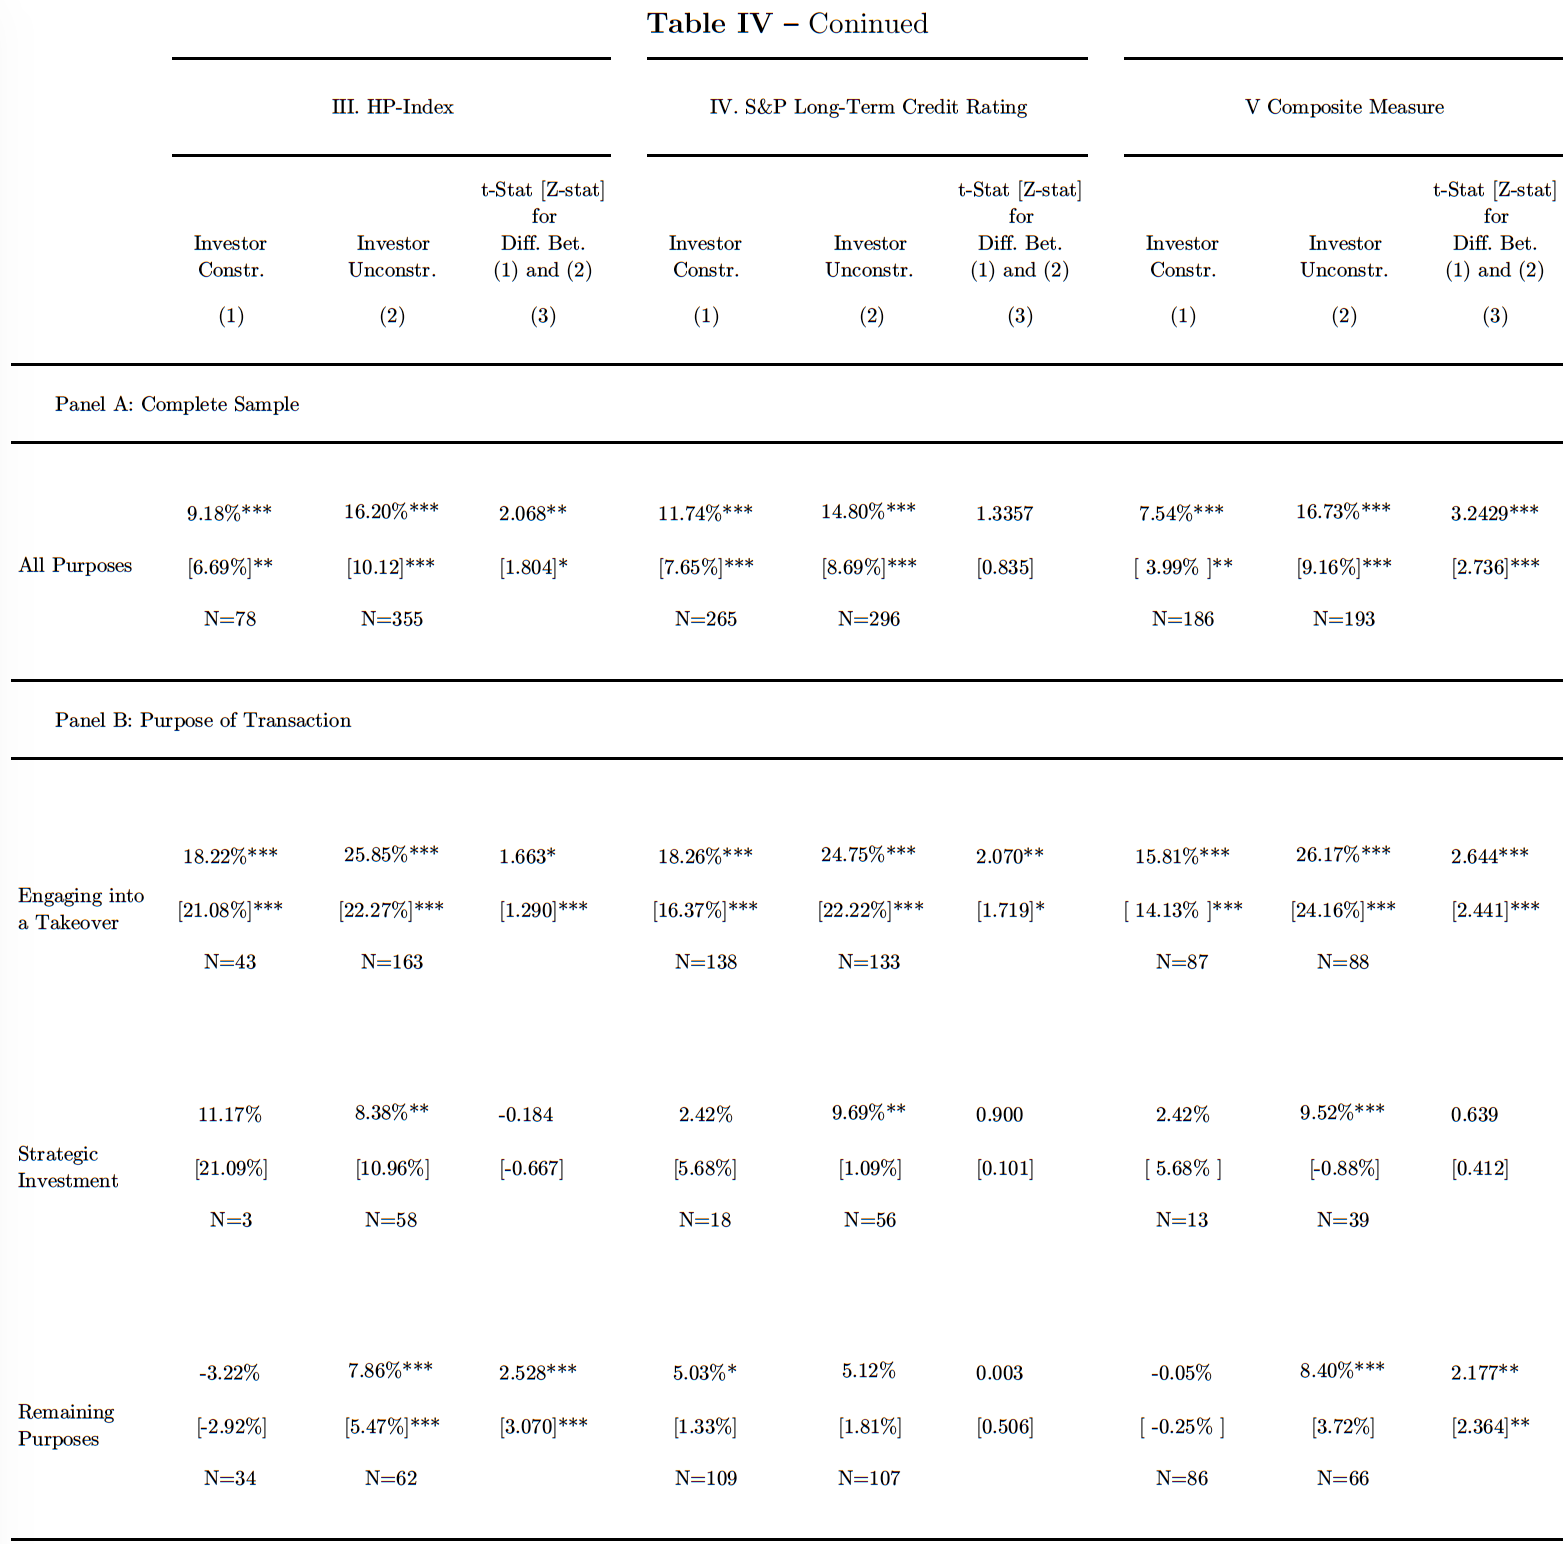
\includegraphics{Ar_measure2_montag_copy}
	\end{adjustbox}
\end{table}  
Targets subject to filings with the purpose of strategic investments have a 7.92\% CAR, significant at the 5\% level which is a similar market reaction to the one observed by \citet[p.]{Allen2000} who find abnormal returns of 6.9\% in response to strategic announcements. For the reason that the sample consists of only 74 filings with the transaction purpose of a strategic investment, performing tests and deriving conclusions on the economic and statistical significance in differences is problematic. The issue becomes even more demanding when  further splitting filings into the sub-samples of each measure, as they become smaller and tests start to loose their power. Subsequently, there are only 16, 15, 18 and 13 observations in the four samples of constrained investors from the WW-Index, dividend payout ratio, the credit rating and the composite measure and just three for the HP-Index. Samples of the Whited-Wu index and the investor's credit rating present differences in mean CAR's matching with previous findings. Targets of financially constrained investors have average abnormal returns below those of financially unconstrained investors, yet the difference is not significant. These findings are supported by the composite measure but when considering average abnormal returns from the sub-samples of the investor's dividend payout ratio and the HP-Index, results differ. With regards to both measures, targets of financially constrained investors now have higher abnormal returns when compared to those of financially unconstrained investors. Concluding, strategic filings do not allow for valid inferences among constrained and unconstrained investors. The evidence is twofold, as three measures support the proposition that financial constraints matter for strategic filings, whereas the other two measures disprove it.\par
With regards to the remaining purposes of transaction, the average cumulative abnormal return is 5.07\% for the [-10,3] event window. This means that filings disclosed in the process of strategic investments, and engaging into a takeover, lead to the strongest market reactions. This is conceivable, as the potential value improvement for the target should be the largest in the presence of takeover premiums and strategic synergies. When looking at abnormal returns for sub-samples of the Whited-Wu index, targets of financially constrained investors lose -0.49\% whereas targets of unconstrained investors gain 8.31\% in value. The difference is significant from zero at the 5\% level and similar conclusions can be drawn from the sub-samples formed by the HP-index. Targets of constrained investor lose -3.22\% whereas targets of constrained investors gain 7.86\% in value. While the difference in average cumulative abnormal returns is now significant at the 1\% level it further supports the proposition that financial constraints of the investor matter, independent of the transaction purpose\par
Concluding, Table IV provides further answers to the investigation on whether financial constraints of corporate activist investors matter. The univariate analysis shows that both, across different measures of financial constraints and transaction purposes, the difference in abnormal returns is existent and significant. Irregularities are only evident for strategic filings, but here too does the Whited-Wu index show differences in abnormal returns. The different measures of financial constraints yield matching results and have categorical power when analyzing the targets' cumulative abnormal returns. This in turn supports the hypothesis that financial constraints of corporate activist investors matter. 
% The difference is the greatest among targets of constrained and unconstrained investors and of those missing a credit rating and those having one. For both measure, the difference is statistically significant at the 1\% level. Strikingly, targets of investor identified to be in financial distress have a mean CAR of 25.65\%, 4\% higher when compared to undistressed firms. An explanation might be that the distressed companies equity claimants are up for a "gamble of ressurection" \citep[p.451]{Bhagat2005} in which they hope conditions may improve and the market interprets this behavior as promising for the target. For all measures, excluding the $Z$-score, is the difference in abnormal returns between the two sub-samples statistically significant at the 1\% level and targets of investor in the favorable state gain more

\section{Cross Sectional Variation of Abnormal Returns}

\noindent Equally important as the average abnormal return subject of analysis in the previous section is its cross-sectional variation because it reflects the heterogeneity in market perceptions regarding the expected value generated by activism. The advantage is that it allows to draw \emph{ceteris paribus} conclusions, which simple t-tests of means cannot do \citep[p.111]{Khatami2014}. Does the market's perceived value improvement for the target depend on the investor? What is the relationship between financially constrained investors and target's abnormal returns among the sample of Schedule 13(D) filings?
Table V reports the results from ordinary least squared regressions exploring the cross-sectional variation in market response to corporate activist investors' Schedule 13(D) filings. The regression is constructed as follows 

\begin{equation}
	CAR_{i}=\beta_{0}+\beta_{1}FC_{i}+\sum_{k=1}^{n}\beta_{k}+X_{k,i}+\epsilon_{i}
\end{equation}
where the dependent variable $CAR_{i}$ is the cumulative abnormal return in the [-10,3] event window for target $i$. This means the regression is based on cross-sectional data, as for each filing (event) there exists one observation of abnormal returns, the cumulative abnormal return for target $i$. FC is a dummy variable equal to 1, if in filing $i$ the investor is classified to be financially constrained and zero if otherwise and corresponds to each of the measures. Hence for each measure -- Whited-Wu index, HP-Index, dividend payout ratio, credit rating and composite measure -- the regression is performed separately. This leads to five regressions in Table V. Appendix C presents a table of several regressions for each measure of financial constraints to provide robustness of the results. $X_{k,i}$ represents a vector of control variables of filing, investor and target characteristics, with \emph{takeover} and \emph{strategic} being equal to one if the transaction purpose was due to engaging into a takeover or strategic investment. To minimize the risk of spurious inference, proxies for the business cycle \emph{recession}, and both the investor's and target's Tobin's Q are included. \emph{Recession} is a dummy variable equal to one if the filing was disclosed either in the year 2001 (early 2000s recession) or in the years from 2007-2009 (Great Recession) and zero otherwise. In addition, the regression controls for the \emph{ROA} and \emph{Cash flow from Operations to Assets} for both investor and target and the \emph{Relative Size}, defined as the natural logarithm of target total assets divided by bidder total assets. The variable \emph{Relative Size} is included because small firms are more vulnerable to capital market imperfections  as they are less well known \citep[p.2004]{Almeida2004}. Additionally, the regressions control for the gap between the datadate of the investor's fundamentals and the filing date of the Schedule 13(D). In a last step, all regressions control for both (fixed effects), the investor's and target's industry, defined by Fama \& French's 17 Industry classification code, to remove unobserved time-varying industry shocks.\footnote{To prevent over-classification of the model, the 17 rather than the 48 industry classification is used.} The effect size of each independent variable is in original units of the dependent variable, thus can be interpreted as the effect in abnormal returns.\par
\begin{table}[!htbp]
	\centering
	\captionsetup{textformat=empty,labelformat=blank}
	\caption{Relation between Abnormal Returns and Financial Constraints}
	\textbf{Table V}\par\medskip
	\large\textbf{Relation between Abnormal Returns and Financial Constraints}\par\medskip
	\justifying
	\footnotesize\noindent\setstretch{1.0} The dependent variable is the cumulative abnormal return the (-10,+3)-day window around the Schedule 13(D) filing date. The main regressors are the financial constraints measures as defined in Section 3. All regressions control for the \emph{Relative Size} defined as the natural logarithm of target total assets divided by bidder total assets and is taken from \citet[p.112]{Khatami2014}. The two dummy variables \emph{Takeover} and \emph{Strategic}, equal one if the purpose of transaction is engaging into a takeover or a strategic investment, zero otherwise. \emph{Recession} equals one if the filing was disclosed in 2001 or in the period from 2007-2009, zero otherwise. Target's and investor's \emph{CF from Operations / At}, the ratio of cash-flow from operations to total assets, \emph{Tobin's Q} and ROA, the ratio of EBITDA to total assets. Appendix A list measure definitions and Appendix B purpose definitions. All data are winsorized at the 1\% and 99\% levels. All $t$-statistics adjust for heteroskedasticity. *, ** and *** indicate statistical significance at the 10\%, 5\% and 1\% levels.\par\medskip									
	\begin{adjustbox}{max width=\textwidth}
		\begin{tabular}{lccccc}
			\multicolumn{6}{c}{} \\ \hline
			\\
			VARIABLES & (1) &(2) & (3)& (4) & (5)\\ \hline
			 &  &  &  &  &  \\
			Whited--Wu Index & -0.1057*** &  &  &  &  \\
			 & (-3.2772) &  &  &  &  \\
			HP--Indicator &  & -0.0401 &  &  &  \\
			 &  & (-0.9568) &  &  &  \\
			Dividend Payout Ratio &  &  & -0.0512* &  &  \\
			 &  &  & (-1.9301) &  &  \\
			Credit Rating &  &  &  & -0.0024 &  \\
			 &  &  &  & (-0.0886) &  \\
			Composite Measure &  &  &  &  & -0.0896*** \\
			 &  &  &  &  & (-2.6211) \\
			Relative Size & -0.2740*** & -0.2381*** & -0.2787*** & -0.2988*** & -0.1954*** \\
			 & (-4.0921) & (-3.7063) & (-4.4917) & (-5.0513) & (-2.8137) \\
			Takeover & 0.1633*** & 0.1922*** & 0.1746*** & 0.1642*** & 0.1860*** \\
			 & (5.5895) & (6.7514) & (6.5086) & (6.6743) & (5.8871) \\
			Strategic & 0.0322 & 0.0503 & -0.0000 & 0.0340 & 0.0270 \\
			 & (0.6507) & (1.0405) & (-0.0005) & (0.7773) & (0.4488) \\
			Recession & 0.0468 & 0.0230 & -0.0102 & -0.0020 & 0.0035 \\
			 & (1.2765) & (0.6478) & (-0.3174) & (-0.0656) & (0.0927) \\
			CF from Operations / AT & -0.0090 & 0.2328 & 0.1014 & 0.2373 & 0.3783** \\
			 & (-0.0357) & (1.2730) & (0.6134) & (1.5015) & (1.9960) \\
			CF from Operations / AT (Target) & 0.2033** & 0.0261 & 0.0734 & -0.0791 & -0.1954** \\
			 & (2.1407) & (0.2480) & (0.7216) & (-0.7740) & (-2.3234) \\
			Tobin's Q & -0.0075 & -0.0100 & -0.0150 & -0.0068 & -0.0085 \\
			 & (-0.6078) & (-0.9737) & (-1.3263) & (-0.7061) & (-0.7065) \\
			Tobin's Q (Target) & -0.0211*** & -0.0249*** & -0.0221*** & -0.0232*** & -0.0281*** \\
			 & (-3.2486) & (-3.5823) & (-3.7300) & (-3.8154) & (-3.8099) \\
			ROA & -0.1490 & -0.2766 & -0.1043 & -0.2424 & -0.4863** \\
			 & (-0.6313) & (-1.3729) & (-0.6034) & (-1.4534) & (-2.3513) \\
			ROA (Target) & -0.2554** & -0.0348 & -0.0834 & 0.0799 & 0.2069* \\
			 & (-2.0987) & (-0.2746) & (-0.6648) & (0.6895) & (1.6910) \\
			 &  &  &  &  &  \\
			Constant & 0.3212*** & 0.2671*** & 0.3530*** & 0.3145*** & 0.2778*** \\
			 & (3.5804) & (3.0333) & (3.9055) & (3.7851) & (2.8794) \\
			 &  &  &  &  &  \\
			Observations & 401 & 403 & 458 & 521 & 358 \\
			 R-squared & 0.2829 & 0.2791 & 0.2621 & 0.2430 & 0.2844 \\ \hline
			\multicolumn{6}{c}{ t-statistics adjusted for heteroskedasticity in parentheses} \\
			\multicolumn{6}{c}{ ***, **, *, report statistical significance at the 1\%, 5\% and 10\% levels, respectively}\\
			\end{tabular}			
	\end{adjustbox}
\end{table}
Turning first to Column (1) and keeping everything else equal, corporate activism of financially constrained investors identified by the Whited-Wu index, generates abnormal returns 10.57\% lower when compared to activism by unconstrained investors. The coefficient of the Whited-Wu dummy variable is significant at the 1\% level, implying that investor's financial constraints matter when the market reacts to Schedule 13(D) filings and there is cross-sectional dependency between abnormal returns and the investor's financial condition. This is matching with previous results from the univariate analysis, where targets of financially constrained investors had average abnormal returns 10\% lower compared to targets of unconstrained investors. Keeping everything else equal, targets subject to a filing with the purpose of engaging into a takeover experience abnormal returns 16.33\% higher when compared to the reference group, namely the remaining transaction purposes. While the latter is significant at the 1\% level, the 3.22\% increase in abnormal returns for targets of strategic Schedule 13(D) filings is not significant at any conventional level. Considering the regression also controls for the transaction purposes, the 10\% decrease in abnormal returns for targets of financially constrained investors is independent from the filing's transaction purpose. This supports the proposition that financial constraints matter, independent from the filing's transaction purpose.\par
Furthermore, relative size is an important determinant of the market's perceived value improvement for the target, and apparent across all regressions. If investor and target have the same size, abnormal returns are reduced by 27.40\%. The larger the investing corporation and the smaller the target, the smaller is the reduction in abnormal returns. As smaller firms have less excess to external finance, this could be further evidence in favor of the hypothesis that financial constraints matter \citep[p.15]{heller2015}.\par
Heading to Column (2), the HP-index is used to identify financially constrained investors. As the coefficient is not significant, it follows that the null hypothesis, that is to say the investor's financial constraints have no effect on the target's abnormal returns, cannot be rejected. Although this fails to further verify the proposition that financial constraints matter, it in turn does not oppose it. When testing the regression with different control variables for robustness, the coefficient of the HP-index dummy stays significant at the 5\% level as long as relative size is excluded. This indicates that beyond the size-effect, the HP-Indicator might only have modest explanatory power in the sample of corporate activist investors. Similar to the preceding results, relative size has a large effect on the target's abnormal returns.\par
Column (3) provides further evidence that financial constraints of corporate activist investors matter, when the market perceives the value improvement for the target. Applying the investor's dividend payout ratio as a measure for financially constrained and unconstrained investors, targets of financially constrained investors experience lower abnormal returns. Other things equal and with a coefficient significant at the 10\% level, targets of financially constrained investors gain 5.12\% less. This is matching with the results from the regression using the Whited-Wu index and supports the results.\par
Following, Column (4) presents the results of the regression using the investor's credit rating as a measure of financial constraints. Although targets of investors without a credit rating gain less, the coefficient looses its significance when including the investor's size in the regression. This is similar to the HP-Index and might result from the conjoint relation between size and credit rating. Additionally, the lack of explanatory power might be due to the credit rating's classification process as a measure of financial constraints. In contrast to the other measures, it classifies almost half of the investors as financially constrained, thereby potentially introducing bias in which financially unconstrained corporations are falsely identified to be financially constrained.\par
Lastly, Table V presents the regression using the composite measure for financial constraints. Column 5 suggests that constrained investor's, identified by the composite measure, have a negative effect on the target's gains. The effect can be placed between the effect of regressions (1) and (3) as targets of financially constrained investors experience 8.96\% lower abnormal returns, other things equal. Considering the coefficient is significant at the 1\% level, this directly supports the other regressions and thereby the proposition that financial constraints matter.\par
The cross sectional regressions support previous findings on financial constraints and abnormal returns. They show, that other things equal, a negative relation between investor's financial constraints and target's abnormal returns exists. Financially constrained investors classified by the Whited-Wu index have the strongest negative impact on the target's abnormal returns. In the [-10,3] window around the Schedule 13(D) filing date, their targets gain 10\% less. When sorted by their dividend payout ratio, their targets experience a 5\% smaller value improvement. This findings are supported by the regression using the composite measure where the effect is 8.96\%. This means, the market assesses financially constrained investors to be less value generating for the target. Yet the evidence is not definitive, as only three measures show a significant influence on the target's abnormal returns. Table V further verifies the proposition, that financial constraints of investors matter, independent from the filing's transaction purpose, and are thus valid determinants across all Schedule 13(D) filings. Ultimately, the cross-sectional relation between abnormal returns and financial constraints shows that the target's perceived value improvement is dependent on the corporate activist investor and financial constraints matter.
\pagebreak

\section{Conclusion}
\noindent This thesis analyzes the relationship between financial constraints of corporate activist investors and target's abnormal returns among the sample of Schedule 13(D) filings in the United States. The term corporate activist investor speaks for the instance, in which corporations disclose a Schedule 13(D) filing after taking a stake of at least 5\% of beneficial ownership in a company. Schedule 13(D) filings have enjoyed wide spread attention, particularly when initiated by institutional investors. Recent literature has addressed their interests and motives, the market reactions and target characteristics. Yet a detailed investigation of Schedule 13(D) filings disclosed by corporate activist investors has not been conducted. Using a sample of Schedule 13(D) filings disclosed by corporations from 1996-2016, this thesis adds to the literature in providing evidence that announcements of such corporate investments result in significant gains for the target. By estimating abnormal returns with the market model, the average abnormal return in the [-10,3] window for the complete sample is 13\%, applying and confirming existing evidence, that such investments are perceived as actual value improvements for the target. The filings' transaction purposes are matching with findings on different types of corporate equity ownership, namely in the form of actively engaging into proceedings such as takeovers, strategic partnerships or overcoming informational barriers.\par 
The thesis' research focus is concerned with the relationship between investor's financial constraints and the abnormal returns for the target. The results suggest that financially constrained investors, likewise their restricted access to external financing, is related to the market's evaluation of the target's potential gains. Using a variety of financial constraint measures to identify financially constrained and unconstrained investors, the univariate analysis shows that targets of constrained investors experience significantly lower abnormal returns in response to Schedule 13(D) filings. The difference is apparent, both across various event-windows and different transaction purposes, showing that financial constraints matter on the whole. The multivariate analysis confirms that, other things equal, targets of financially constrained investors experience considerably lower abnormal returns compared to targets of unconstrained investors resulting in a negative relationship between investor's financial constraints and target's abnormal returns. The evidence on smaller abnormal returns for targets of financially constrained investors allows to draw the conclusion, that financial constraints of corporate activist investors matter.\par 
The evidence could be further supported by implementing improved proxies for the expected development of the investor's financial constraints. As such expectations are often founded on historic trends, one approach would be to analyse the development in financial constraints for the investor over several years preceding the Schedule 13(D) filing and thereby drawing further conclusions on the market's expectations for the investor and the target. Beyond the restricted access to external financing, the multivariate analysis shows that the investor's size and the relation between target and investor are important determinants when analyzing the target's abnormal returns. This indicates that a deepened investigation of alternative characteristics of both corporate activist investors and targets could advance research. As this thesis analyzes the market reaction to American filings of beneficial ownership, enlarging the scope of analysis to European and even Emerging markets could further add to the area of corporate activist investments.
\cleardoublepage
\pagenumbering{roman}
\setcounter{page}{\thesavepage}
\addcontentsline{toc}{section}{References}

\printbibliography[title=References]

\section*{Other Sources}
	\begin{itemize}
	\renewcommand\labelitemi{--}

		\item CRSP Stocks. (1995-2016). Available: Center for Research in Security Prices. Graduate School of Business. University of Chicago. Retrieved from Wharton Research Data Services.
		\item Compustat [Annual Data]. (1993-2016). Available: Standard \& Poor's/Compustat. Retrieved from Wharton Research Data Services.
		\item StataCorp. 2013. Stata Statistical Software: Release 13. College Station, TX: StataCorp LP.
		\item U.S. Securities and Exchange Commission. (2018). EDGAR Database.
	\end{itemize}

\cleardoublepage	
\begin{appendices}
\renewcommand{\appendixname}{Appendix}

\section*{Appendix A\indent Financial Constraints Measures \& Variables}
  
	\subsection*{Whited--Wu Index}
	\noindent Used from \citet[p.543]{Whited2006} and following \citet[p.305]{Farre-Mensa2016} the Whited-Wu index is calculated as:
		\begin{equation*}
		WW=-0.091X_{1}-0.062X_{2}+0.021X_{3}-0.044X_{4}+0.102X_{5}-0.035X_{6}
		\end{equation*}
	where
	\begin{itemize}
	\renewcommand\labelitemi{}
		\item $X_{1}$ is the ratio of cash flow to assets defined as the sum of income before extraordinary items and depreciation and amortization divided by total assets $\frac{ib+dp}{at}$
		\item $X_{2}$ is an indicator set to one if the firm pays a dividend, likewise if the sum of common and preferred dividends paid is positive, zero otherwise $dvp+dvc>0$
		\item $X_{3}$ is the ratio of long-term debt to total assets $\frac{dltt}{at}$
		\item $X_{4}$ is the size of the investor defined as the natural logarithm of total assets $log(at)$
		\item $X_{5}$ is the average industry sales growth, estimated for each three digit SIC industry and each year separately $\frac{SALE_{t}}{SALE_{t-1}}$
		\item $X_{6}$ is the investor's sales growth $\frac{SALE}{SALE_{t-1}}$
	\end{itemize}

	\noindent and all variables in italics are Compustat data items. Following convention, the index is calculated for all firms on Compustat and firms are then sorted into terciles based on their index value. Firms in the top tercile are coded as constrained and those in the bottom tercile are coded as unconstrained \citep[p.306]{Farre-Mensa2016}. 

	\subsection*{Dividend Payout Ratio}
	\noindent Following \citet[p.119]{Khatami2014} and \citet[p.1789]{Almeida2004}, the investor's dividend payout ratio is defined as the two-year average of the dividend payout ratio from the two preceeding annual reports at each point in time.\\
	The yearly dividend payout ratio is defined as the sum of dividends ($dvp+dvc$) plus stock repurchases (total expenditure on the purchase of common and preferred stocks $prstkc$) minus any reduction in the value of net number of preferred stocks outstanding (redemption value $pstkrv$) divided by operating income ($\frac{ib}{at}$) as in \citet[p.369]{Jagannathan2000}. Further, following \citet[p.119]{Khatami2014} and \citet[p.1923]{hadlock2010} dividend payout ratios are set equal to 1 if they are above 1 and if a firm has negative operating income and positive dividends. After computing the two-year average payout ratio for all firms on Compustat, firms are sorted into terciles based on their annual payout distribution. Firms in the bottom (top) tercile are coded constrained (unconstrained). 

	\subsection*{HP / SA -- Index}
	\noindent Following \citet[p.1929]{hadlock2010} and \citet[p.119]{Khatami2014} the index is calculated as: $HP=-0.737*Size+0.043*Size^{2}-0.040*Age$ where size is the log of inflation adjusted (to 2004) book assets and age is the number of years the firm has been on Compustat with a non-missing stock price. In calculating the index, size is replaced with log(\$4.5 billion) and age with 37 years if the actual values exceed these thresholds \citep[p.1929]{hadlock2010}. After computing the HP index for all companies on Compustat, the firms are sorted into terciles based on their annual index values. Firms in the top tercile are coded as constrained and those in the bottom tercile are conded as unconstrained \citep[p.306]{Farre-Mensa2016}.

	\subsection*{Rating-Indicator}
	\noindent Following \citet[p.18]{heller2015}, \citet[p.1790]{Almeida2004} and \citet[p.305]{Farre-Mensa2016} firms that have a S\&P domestic long-term issuer credit rating at least 3 months prior to the Schedule 13(D) filing date are considered to be financially unconstrained. In contrary, firms missing such a credit rating are considered to be financially constrained. The data are obtained from Compustat (variable \emph{splticrm})
	\subsection*{Other Variables}

	\begin{itemize}
	\renewcommand\labelitemi{--}
		\item Return on assets $\frac{ebitda}{at}$
		\item Cash flow from operations to total assets $\frac{oancf}{at}$
		\item Cash and short-term investments to total assets $\frac{che}{at}$
		\item Cash to total assets $\frac{ch}{at}$
		\item Book Leverage \citep[p.1440]{MacKay2005} $\frac{dltt+dlc}{at}$
		\item Short-term debt to total assets $\frac{dlc}{at}$ 
		\item Long-term debt to total assets $\frac{dltt}{at}$
		\item Market value of equity $prcc_f*csho$
		\item Size of the firm $log(at)$
		\item Tobin's Q \citep[p.120]{Khatami2014} $\frac{at-ceq-txdb+csho*prcc_c}{at}$
	\end{itemize}


\section*{Appendix B\indent Categorization Purpose of Transaction}

\noindent The following definitions are explanatory excerpts of Schedule 13(D) filings from the sample. Based on these descriptions the filing's transaction purpose was identified. Following, the Reporting Person is the investor disclosing the Schedule 13(D) wheras the Issuer is the company subject to the filing. 
\begin{enumerate}
	

\item Merger: "the Company entered into the Merger Agreement with the Reporting Person and Merger Sub, pursuant to which the Reporting Person will acquire all of the outstanding equity interests of the Company."

\item Tender Offer: "The Reporting Person announced its intention to commence a partial cash tender offer for up to \emph{number of} shares of Common Stock at a price of \emph{\$ price} net per share"

\item Hostile Takeover: "The Shares have been acquired by the Reporting Persons with a view to ultimately acquiring  control of the Issuer  pursuant to a merger with, or  acquisition of additional  stock  by,  the Reporting Person  or one of its  subsidiaries. [...]
% Such  merger  or acquisition would likely result in changes to the present Board of Directors and management  of the  Company,  and  might  result  in  changes  in the  Company's capitalization and dividend policy, business, corporate structure and governing documents. 
The Reporting Person has contacted the Chairman of the Board of the Issuer and expressed an interest in acquiring the Company and expects to have further discussions  with management of the Issuer."

\item Investment Opportunity while Actively Monitoring the Target: "The primary purpose of the Reporting Person's acquisition of the Common Stock is for investment. The Reporting Person believes that at this time, the Common Stock represents an attractive investment opportunity. Although it has no current intention to do so, at some time in the future the Reporting Person may decide that it is desirable to seek to acquire the Issuer or seek to control or otherwise influence the management and policies of the Issuer."

\item Alliance Agreement: "The purpose of the transaction is for investment and to establish a long term distribution alliance between the Reporting Person and the Issuer."

\item License Agreement: "As set forth, the Shares were purchased on  in connection with the Development and License Agreement between the Issuer and the Reporting Person."

\item Joint Venture: "The Reporting Person acquired shared voting and investment power over the Contributed Shares in connection with the formation of the joint venture with the Issuer."

\item Engaging into a Proxy Fight: [...] nominating \emph{Person} and \emph{Person} to be elected by holders of the Shares to the Board of Directors of the Issuer (the “Board”) at the annual meeting of stockholders of the Issuer, or any other meeting of stockholders held in lieu thereof, and any adjournments, postponements, reschedulings or continuations thereof (the “Annual Meeting”). The Reporting Persons reserve the right to take all action they deem appropriate to obtain Board representation. 

\item Investor is Subject to Merger: "At the effective time of the Merger (the “Effective Time”), the separate existence of Merger Sub will cease and the Reporting Person will continue as the Surviving corporation and as a wholly owned subsidiary of the Issuer. Each holder of outstanding common stock of the Reporting Person, par value \emph{\$ per share} will receive, in exchange for each share of the Reporting Person's Common Stock held by such holder, \emph{amount} of a share of the Issuer Common Stock (the “Exchange Ratio”).

\item Issuer Financing: "The purpose of the purchase of the Stock was to provide the Issuer with immediately available funds to address its urgent liquidity needs in exchange for an equity interest in the Issuer."
\end{enumerate}

				\begin{comment}
				\section{Event Study}

				\noindent In order to compute the abnormal returns $AR_{i,t}$ for security $i$ at time $t$ in \eqref{eq:1} the market model is used. For the expected return it assumes a constant and linear relation between the observed returns $R_{i\tau}$ and the return of a market index $R_{m\tau}$. The parameters are estimated by ordinary least squares regressions based on estimation-window observations \citep[p.210]{Corrado2011}. The value-weighted NYSE/Amex/Nasdaq index from CRSP is used as the market return $R_{M\tau}$.

							\begin{equation*}
								R_{i,\tau}=\alpha_{i}+\beta_{i}R_{M,\tau}+\epsilon_{i,\tau}
							\end{equation*}
							with 
							\begin{equation*}
								E[\epsilon_{i,\tau}]=0
							\end{equation*}
							and 
							\begin{equation*}
								Var[\epsilon_{i,\tau}]=\sigma^2_{i,\tau}
							\end{equation*}
							This yields the abnormal return $AR_{i,\tau}$
							\begin{equation}
								AR_{i,\tau}=R_{i,\tau}-(\hat{\alpha_{i}}+\hat{\beta_{i}}R_{M,\tau})
							\end{equation}
				\end{comment}

\section*{ Appendix C\indent Robustness of the Regressions}
\noindent Appendix C shows one table for the cross sectional variation of abnormal returns for each of the five measures of financial constraints. The ordinary least squared regressions in Tables 1-5 have the aim to provide robustness for the analysis of section 5and all variables definitions are equal to the ones presented in Section 5. The regression tables are constructed as follows: Independent of other control variables, all regressions control for the target's and investor's indutry (Fama \& French 17 industry classification) and the gap (in months) between the reported datadate and the Schedule 13(D) filing date. The regression of Column (1) in each table includes the measure of financial constraints as the only regressor. The regression in Column (2) further adds the purposes of transaction -- the dummy variables \emph{Takeover} or \emph{Strategic}. The regression in Column (3) includes investor characteristics \emph{Size}, \emph{Cash-Flow from Operations to Assets}, \emph{Return on Assets} and \emph{Tobin's Q} and the dummy variable \emph{Recession}. Equivalently, the regression of Column (4) includes as regressors target characteristics \emph{Size Target}, \emph{Cash-Flow from Operations to Assets Target}, \emph{Return on Assets Target} and \emph{Tobin's Q Target} and the dummy variable \emph{Recession}. The last regression in Column (4) includes all above mentioned variables as regressors but replaces the target's and investor's size with the variable \emph{Relative Size}.

\begin{table}[!htbp]
	\centering
	\textbf{Table A1}\par\medskip
	\large\textbf{Relation between Abnormal Returns and Financial Constraints -- Whited-Wu Index}\par\medskip
	\justifying
	\footnotesize\noindent\setstretch{1.0} The dependent variable is the cumulative abnormal return the (-10,+3)-day window around the Schedule 13(D) filing date. The main regressor is the dummy variabe for financially constrained and unconstrained investors of the Whited-Wu index. All regressions control for the \emph{Relative Size} defined as the natural logarithm of target total assets divided by bidder total assets and is taken from \citet[p.112]{Khatami2014}. The two dummy variables \emph{Takeover} and \emph{Strategic}, equal one if the purpose of transaction is engaging into a takeover or a strategic investment, zero otherwise. \emph{Recession} equals one if the filing was disclosed in 2001 or in the period from 2007-2009, zero otherwise. Target's and investor's \emph{CF from Operations / At}, the ratio of cash-flow from operations to total assets, \emph{Tobin's Q} and ROA, the ratio of EBITDA to total assets. All data are winsorized at the 1\% and 99\% levels. All $t$-statistics adjust for heteroskedasticity. *, ** and *** indicate statistical significance at the 10\%, 5\% and 1\% levels.\par\medskip
	\begin{adjustbox}{max width=\textwidth}
		\begin{tabular}{lccccc} \hline
			\\
		   VARIABLES & (1) & (2) & (3) & (4) & (5) \\ \hline
			&  &  &  &  &  \\
		   Whited-Wu Indicator & -0.1249*** & -0.1138*** & -0.1019*** & -0.1533*** & -0.1057*** \\
			& (-3.5975) & (-3.3751) & (-2.6724) & (-4.4790) & (-3.2772) \\
		   Takeover &  & 0.1702*** &  &  & 0.1633*** \\
			&  & (5.9406) &  &  & (5.5895) \\
		   Strategic &  & 0.0345 &  &  & 0.0322 \\
			&  & (0.7911) &  &  & (0.6507) \\
		   Size &  &  & 0.0151* &  &  \\
			&  &  & (1.7099) &  &  \\
		   Size (Target) &  &  &  & -0.0252** &  \\
			&  &  &  & (-2.5246) &  \\
		   CF from Operations / Assets &  &  & -0.0095 &  & -0.0090 \\
			&  &  & (-0.0562) &  & (-0.0357) \\
		   CF from Operations / Assets (Target) &  &  &  & 0.1576 & 0.2033** \\
			&  &  &  & (1.5614) & (2.1407) \\
		   ROA &  &  & -0.0893 &  & -0.1490 \\
			&  &  & (-0.5084) &  & (-0.6313) \\
		   ROA (Target) &  &  &  & -0.1996 & -0.2554** \\
			&  &  &  & (-1.6446) & (-2.0987) \\
		   Tobin's Q &  &  & -0.0152 &  & -0.0075 \\
			&  &  & (-1.0912) &  & (-0.6078) \\
		   Tobin's Q (Target) &  &  &  & -0.0215*** & -0.0211*** \\
			&  &  &  & (-2.7664) & (-3.2486) \\
		   Recession &  &  & 0.0293 & 0.0543 & 0.0468 \\
			&  &  & (0.7591) & (1.3950) & (1.2765) \\
		   Relative Size &  &  &  &  & -0.2740*** \\
			&  &  &  &  & (-4.0921) \\
		   Constant & 0.1509** & 0.0831 & 0.0636 & 0.2904*** & 0.3212*** \\
			& (1.9998) & (1.1572) & (0.4791) & (2.8575) & (3.5804) \\
			&  &  &  &  &  \\
		   Observations & 433 & 433 & 433 & 401 & 401 \\
			R-squared & 0.1178 & 0.1935 & 0.1348 & 0.1921 & 0.2829 \\ \hline
			\multicolumn{6}{c}{ t-statistics adjusted for heteroskedasticity in parentheses} \\
			\multicolumn{6}{c}{ ***, **, *, report statistical significance at the 1\%, 5\% and 10\% levels, respectively}\\
		   \end{tabular}			   
	\end{adjustbox}
\end{table}

\begin{table}[!htbp]
	\centering
	\textbf{Table A2}\par\medskip
	\large\textbf{Relation between Abnormal Returns and Financial Constraints -- HP-Index}\par\medskip
	\justifying
	\footnotesize\noindent\setstretch{1.0} The dependent variable is the cumulative abnormal return the (-10,+3)-day window around the Schedule 13(D) filing date. The main regressor is the dummy variabe for financially constrained and unconstrained investors of the HP-index. All regressions control for the \emph{Relative Size} defined as the natural logarithm of target total assets divided by bidder total assets and is taken from \citet[p.112]{Khatami2014}. The two dummy variables \emph{Takeover} and \emph{Strategic}, equal one if the purpose of transaction is engaging into a takeover or a strategic investment, zero otherwise. \emph{Recession} equals one if the filing was disclosed in 2001 or in the period from 2007-2009, zero otherwise. Target's and investor's \emph{CF from Operations / At}, the ratio of cash-flow from operations to total assets, \emph{Tobin's Q} and ROA, the ratio of EBITDA to total assets. All data are winsorized at the 1\% and 99\% levels. All $t$-statistics adjust for heteroskedasticity. *, ** and *** indicate statistical significance at the 10\%, 5\% and 1\% levels.\par\medskip
	\begin{adjustbox}{max width=\textwidth}
		\begin{tabular}{lccccc} \hline
			\\
		   VARIABLES & (1) & (2) & (3) & (4) & (5) \\ \hline
			&  &  &  &  &  \\
		   HP-Indicator& -0.0811** & -0.0871*** & 0.0055 & -0.1050*** & -0.0401 \\
			& (-2.2107) & (-2.6461) & (0.1069) & (-2.6814) & (-0.9568) \\
		   Takeover &  & 0.2009*** &  &  & 0.1922*** \\
			&  & (7.3501) &  &  & (6.7514) \\
		   Strategic &  & 0.0319 &  &  & 0.0503 \\
			&  & (0.7273) &  &  & (1.0405) \\
		   Size &  &  & 0.0180** &  &  \\
			&  &  & (1.9857) &  &  \\
		   Size (Target) &  &  &  & -0.0232** &  \\
			&  &  &  & (-2.3069) &  \\
		   CF from Operations / Assets &  &  & 0.2625 &  & 0.2328 \\
			&  &  & (1.5360) &  & (1.2730) \\
		   CF from Operations / Assets (Target) &  &  &  & -0.0250 & 0.0261 \\
			&  &  &  & (-0.2487) & (0.2480) \\
		   ROA &  &  & -0.1793 &  & -0.2766 \\
			&  &  & (-0.9891) &  & (-1.3729) \\
		   ROA (Target) &  &  &  & 0.0530 & -0.0348 \\
			&  &  &  & (0.4466) & (-0.2746) \\
		   Tobin's Q &  &  & -0.0114 &  & -0.0100 \\
			&  &  & (-1.0751) &  & (-0.9737) \\
		   Tobin's Q (Target) &  &  &  & -0.0236*** & -0.0249*** \\
			&  &  &  & (-3.1292) & (-3.5823) \\
		   Recession &  &  & -0.0018 & 0.0211 & 0.0230 \\
			&  &  & (-0.0497) & (0.5468) & (0.6478) \\
		   Relative size &  &  &  &  & -0.2381*** \\
			&  &  &  &  & (-3.7063) \\
		   Constant & 0.1090 & 0.0487 & -0.0132 & 0.2406** & 0.2671*** \\
			& (1.5078) & (0.6939) & (-0.1187) & (2.4804) & (3.0333) \\
			&  &  &  &  &  \\
		   Observations & 433 & 433 & 433 & 403 & 403 \\
			R-squared & 0.1127 & 0.2209 & 0.1330 & 0.1557 & 0.2791 \\ \hline
			\multicolumn{6}{c}{ t-statistics adjusted for heteroskedasticity in parentheses} \\
			\multicolumn{6}{c}{ ***, **, *, report statistical significance at the 1\%, 5\% and 10\% levels, respectively}\\
		   \end{tabular}		   
	\end{adjustbox}
\end{table}

\begin{table}[!htbp]
	\centering
	\textbf{Table A3}\par\medskip
	\large\textbf{Relation between Abnormal Returns and Financial Constraints -- Dividend Payout Ratio}\par\medskip
	\justifying
	\footnotesize\noindent\setstretch{1.0} The dependent variable is the cumulative abnormal return the (-10,+3)-day window around the Schedule 13(D) filing date. The main regressor is the dummy variabe for financially constrained and unconstrained investors of the Dividend Payout Ratio. All regressions control for the \emph{Relative Size} defined as the natural logarithm of target total assets divided by bidder total assets and is taken from \citet[p.112]{Khatami2014}. The two dummy variables \emph{Takeover} and \emph{Strategic}, equal one if the purpose of transaction is engaging into a takeover or a strategic investment, zero otherwise. \emph{Recession} equals one if the filing was disclosed in 2001 or in the period from 2007-2009, zero otherwise. Target's and investor's \emph{CF from Operations / At}, the ratio of cash-flow from operations to total assets, \emph{Tobin's Q} and ROA, the ratio of EBITDA to total assets. All data are winsorized at the 1\% and 99\% levels. All $t$-statistics adjust for heteroskedasticity. *, ** and *** indicate statistical significance at the 10\%, 5\% and 1\% levels.\par\medskip
	\begin{adjustbox}{max width=\textwidth}
		\begin{tabular}{lccccc} \hline
			\\
		   VARIABLES & (1) & (2) & (3) & (4) & (5) \\\hline
			&  &  &  &  &  \\
		   Dividend Payout Ratio & -0.0712*** & -0.0644*** & -0.0584** & -0.0845*** & -0.0512* \\
			& (-2.7753) & (-2.6178) & (-2.1100) & (-3.1744) & (-1.9301) \\
		   Takeover &  & 0.1805*** &  &  & 0.1746*** \\
			&  & (6.7945) &  &  & (6.5086) \\
		   Strategic &  & 0.0039 &  &  & -0.0000 \\
			&  & (0.1072) &  &  & (-0.0005) \\
		   Size &  &  & 0.0105 &  &  \\
			&  &  & (1.4256) &  &  \\
		   Size (Target) &  &  &  & -0.0236** &  \\
			&  &  &  & (-2.4845) &  \\
		   CF from Operations / Assets &  &  & 0.1114 &  & 0.1014 \\
			&  &  & (0.7856) &  & (0.6134) \\
		   CF from Operations / Assets (Target) &  &  &  & 0.0365 & 0.0734 \\
			&  &  &  & (0.3538) & (0.7216) \\
		   ROA &  &  & -0.0125 &  & -0.1043 \\
			&  &  & (-0.0783) &  & (-0.6034) \\
		   ROA (Target) &  &  &  & 0.0116 & -0.0834 \\
			&  &  &  & (0.0974) & (-0.6648) \\
		   Tobin's Q &  &  & -0.0203 &  & -0.0150 \\
			&  &  & (-1.6090) &  & (-1.3263) \\
		   Tobin's Q (Target) &  &  &  & -0.0195*** & -0.0221*** \\
			&  &  &  & (-2.6638) & (-3.7300) \\
		   Recession &  &  & -0.0301 & -0.0140 & -0.0102 \\
			&  &  & (-0.8611) & (-0.4114) & (-0.3174) \\
		   Relative Size &  &  &  &  & -0.2787*** \\
			&  &  &  &  & (-4.4917) \\
		   Constant & 0.1217* & 0.0760 & 0.0957 & 0.2698*** & 0.3530*** \\
			& (1.7747) & (1.1753) & (0.8444) & (2.7253) & (3.9055) \\
			&  &  &  &  &  \\
		   Observations & 494 & 494 & 494 & 458 & 458 \\
			R-squared & 0.0915 & 0.1901 & 0.1116 & 0.1363 & 0.2621 \\ \hline
			\multicolumn{6}{c}{ t-statistics adjusted for heteroskedasticity in parentheses} \\
			\multicolumn{6}{c}{ ***, **, *, report statistical significance at the 1\%, 5\% and 10\% levels, respectively}\\
		   \end{tabular}			  
	\end{adjustbox}
\end{table}

\begin{table}[!htbp]
	\centering
	\textbf{Table A4}\par\medskip
	\large\textbf{Relation between Abnormal Returns and Financial Constraints -- Credit Rating}\par\medskip
	\justifying
	\footnotesize\noindent\setstretch{1.0} The dependent variable is the cumulative abnormal return the (-10,+3)-day window around the Schedule 13(D) filing date. The main regressor is the dummy variabe for financially constrained and unconstrained investors of the Credit Rating. All regressions control for the \emph{Relative Size} defined as the natural logarithm of target total assets divided by bidder total assets and is taken from \citet[p.112]{Khatami2014}. The two dummy variables \emph{Takeover} and \emph{Strategic}, equal one if the purpose of transaction is engaging into a takeover or a strategic investment, zero otherwise. \emph{Recession} equals one if the filing was disclosed in 2001 or in the period from 2007-2009, zero otherwise. Target's and investor's \emph{CF from Operations / At}, the ratio of cash-flow from operations to total assets, \emph{Tobin's Q} and ROA, the ratio of EBITDA to total assets. All data are winsorized at the 1\% and 99\% levels. All $t$-statistics adjust for heteroskedasticity. *, ** and *** indicate statistical significance at the 10\%, 5\% and 1\% levels.\par\medskip
	\begin{adjustbox}{max width=\textwidth}
		\begin{tabular}{lccccc} \hline
			\\
		   VARIABLES & (1) & (2) & (3) & (4) & (5) \\ \hline
			&  &  &  &  &  \\
		   Rating Indicator & -0.0384 & -0.0473** & 0.0394 & -0.0687*** & -0.0024 \\
			& (-1.5268) & (-1.9709) & (1.2414) & (-2.5981) & (-0.0886) \\
		   Takeover &  & 0.1756*** &  &  & 0.1642*** \\
			&  & (7.1822) &  &  & (6.6743) \\
		   Strategic &  & 0.0332 &  &  & 0.0340 \\
			&  & (0.8461) &  &  & (0.7773) \\
		   Size &  &  & 0.0233*** &  &  \\
			&  &  & (2.7400) &  &  \\
		   Size (Target) &  &  &  & -0.0263*** &  \\
			&  &  &  & (-3.0190) &  \\
		   CF from Operations / Assets &  &  & 0.2095 &  & 0.2373 \\
			&  &  & (1.5020) &  & (1.5015) \\
		   CF from Operations / Assets (Target) &  &  &  & -0.0898 & -0.0791 \\
			&  &  &  & (-0.8730) & (-0.7740) \\
		   ROA &  &  & -0.1203 &  & -0.2424 \\
			&  &  & (-0.8123) &  & (-1.4534) \\
		   ROA (Target) &  &  &  & 0.1375 & 0.0799 \\
			&  &  &  & (1.1867) & (0.6895) \\
		   Tobin's Q &  &  & -0.0087 &  & -0.0068 \\
			&  &  & (-0.8128) &  & (-0.7061) \\
		   Tobin's Q (Target) &  &  &  & -0.0215*** & -0.0232*** \\
			&  &  &  & (-3.0478) & (-3.8154) \\
		   Recession &  &  & -0.0066 & 0.0067 & -0.0020 \\
			&  &  & (-0.2070) & (0.2071) & (-0.0656) \\
		   Relative Size &  &  &  &  & -0.2988*** \\
			&  &  &  &  & (-5.0513) \\
		   Constant & 0.1330** & 0.0721 & -0.0648 & 0.2847*** & 0.3145*** \\
			& (1.9757) & (1.1171) & (-0.5928) & (3.1893) & (3.7851) \\
			&  &  &  &  &  \\
		   Observations & 561 & 561 & 561 & 521 & 521 \\
			R-squared & 0.0837 & 0.1702 & 0.1103 & 0.1309 & 0.2430 \\ \hline
			\multicolumn{6}{c}{ t-statistics adjusted for heteroskedasticity in parentheses} \\
			\multicolumn{6}{c}{ ***, **, *, report statistical significance at the 1\%, 5\% and 10\% levels, respectively}\\
		   \end{tabular}			 
	\end{adjustbox}
\end{table}

\begin{table}[!htbp]
	\centering
	\textbf{Table A5}\par\medskip
	\large\textbf{Relation between Abnormal Returns and Financial Constraints -- Composite Measure}\par\medskip
	\justifying
	\footnotesize\noindent\setstretch{1.0} The dependent variable is the cumulative abnormal return the (-10,+3)-day window around the Schedule 13(D) filing date. The main regressor is the dummy variabe for financially constrained and unconstrained investors of the Composite Measure. All regressions control for the \emph{Relative Size} defined as the natural logarithm of target total assets divided by bidder total assets and is taken from \citet[p.112]{Khatami2014}. The two dummy variables \emph{Takeover} and \emph{Strategic}, equal one if the purpose of transaction is engaging into a takeover or a strategic investment, zero otherwise. \emph{Recession} equals one if the filing was disclosed in 2001 or in the period from 2007-2009, zero otherwise. Target's and investor's \emph{CF from Operations / At}, the ratio of cash-flow from operations to total assets, \emph{Tobin's Q} and ROA, the ratio of EBITDA to total assets. All data are winsorized at the 1\% and 99\% levels. All $t$-statistics adjust for heteroskedasticity. *, ** and *** indicate statistical significance at the 10\%, 5\% and 1\% levels.\par\medskip
	\begin{adjustbox}{max width=\textwidth}
		\begin{tabular}{lccccc} \hline
			\\
		   VARIABLES & (1) & (2) & (3) & (4) & (5) \\ \hline
			&  &  &  &  &  \\
		   Composite Measure & -0.1141*** & -0.1165*** & -0.0618 & -0.1329*** & -0.0896*** \\
			& (-3.3940) & (-3.7364) & (-1.4122) & (-3.8445) & (-2.6211) \\
		   Takeover &  & 0.1837*** &  &  & 0.1860*** \\
			&  & (6.0802) &  &  & (5.8871) \\
		   Strategic &  & 0.0107 &  &  & 0.0270 \\
			&  & (0.2030) &  &  & (0.4488) \\
		   Size &  &  & 0.0155 &  &  \\
			&  &  & (1.4705) &  &  \\
		   Size (Target) &  &  &  & -0.0218** &  \\
			&  &  &  & (-2.0053) &  \\
		   CF from Operations / Assets &  &  & 0.2501 &  & 0.3783** \\
			&  &  & (1.4590) &  & (1.9960) \\
		   CF from Operations / Assets (Target) &  &  &  & -0.2008** & -0.1954** \\
			&  &  &  & (-2.2588) & (-2.3234) \\
		   ROA &  &  & -0.2758 &  & -0.4863** \\
			&  &  & (-1.4503) &  & (-2.3513) \\
		   ROA (Target) &  &  &  & 0.2447* & 0.2069* \\
			&  &  &  & (1.9641) & (1.6910) \\
		   Tobin's Q &  &  & -0.0136 &  & -0.0085 \\
			&  &  & (-1.0113) &  & (-0.7065) \\
		   Tobin's Q (Target) &  &  &  & -0.0269*** & -0.0281*** \\
			&  &  &  & (-3.0014) & (-3.8099) \\
		   Recession &  &  & 0.0032 & -0.0078 & 0.0035 \\
			&  &  & (0.0800) & (-0.1947) & (0.0927) \\
		   Relative Size &  &  &  &  & -0.1954*** \\
			&  &  &  &  & (-2.8137) \\
		   Constant & 0.1072 & 0.0757 & 0.0199 & 0.2589** & 0.2778*** \\
			& (1.2853) & (0.9546) & (0.1318) & (2.2638) & (2.8794) \\
			&  &  &  &  &  \\
		   Observations & 379 & 379 & 379 & 358 & 358 \\
			R-squared & 0.1210 & 0.2140 & 0.1384 & 0.1729 & 0.2844 \\ \hline
			\multicolumn{6}{c}{ t-statistics adjusted for heteroskedasticity in parentheses} \\
			\multicolumn{6}{c}{ ***, **, *, report statistical significance at the 1\%, 5\% and 10\% levels, respectively}\\
		   \end{tabular}						
	\end{adjustbox}
\end{table}
\pagebreak


\section*{Appendix D\indent Stata Do-Files}
\noindent The following two do-files comprise the general basis on which the analysis is conducted. The first do-file present the code for computing the measures of financial constraints and second do-file presents the code for the calculation of targets abnormal returns. 
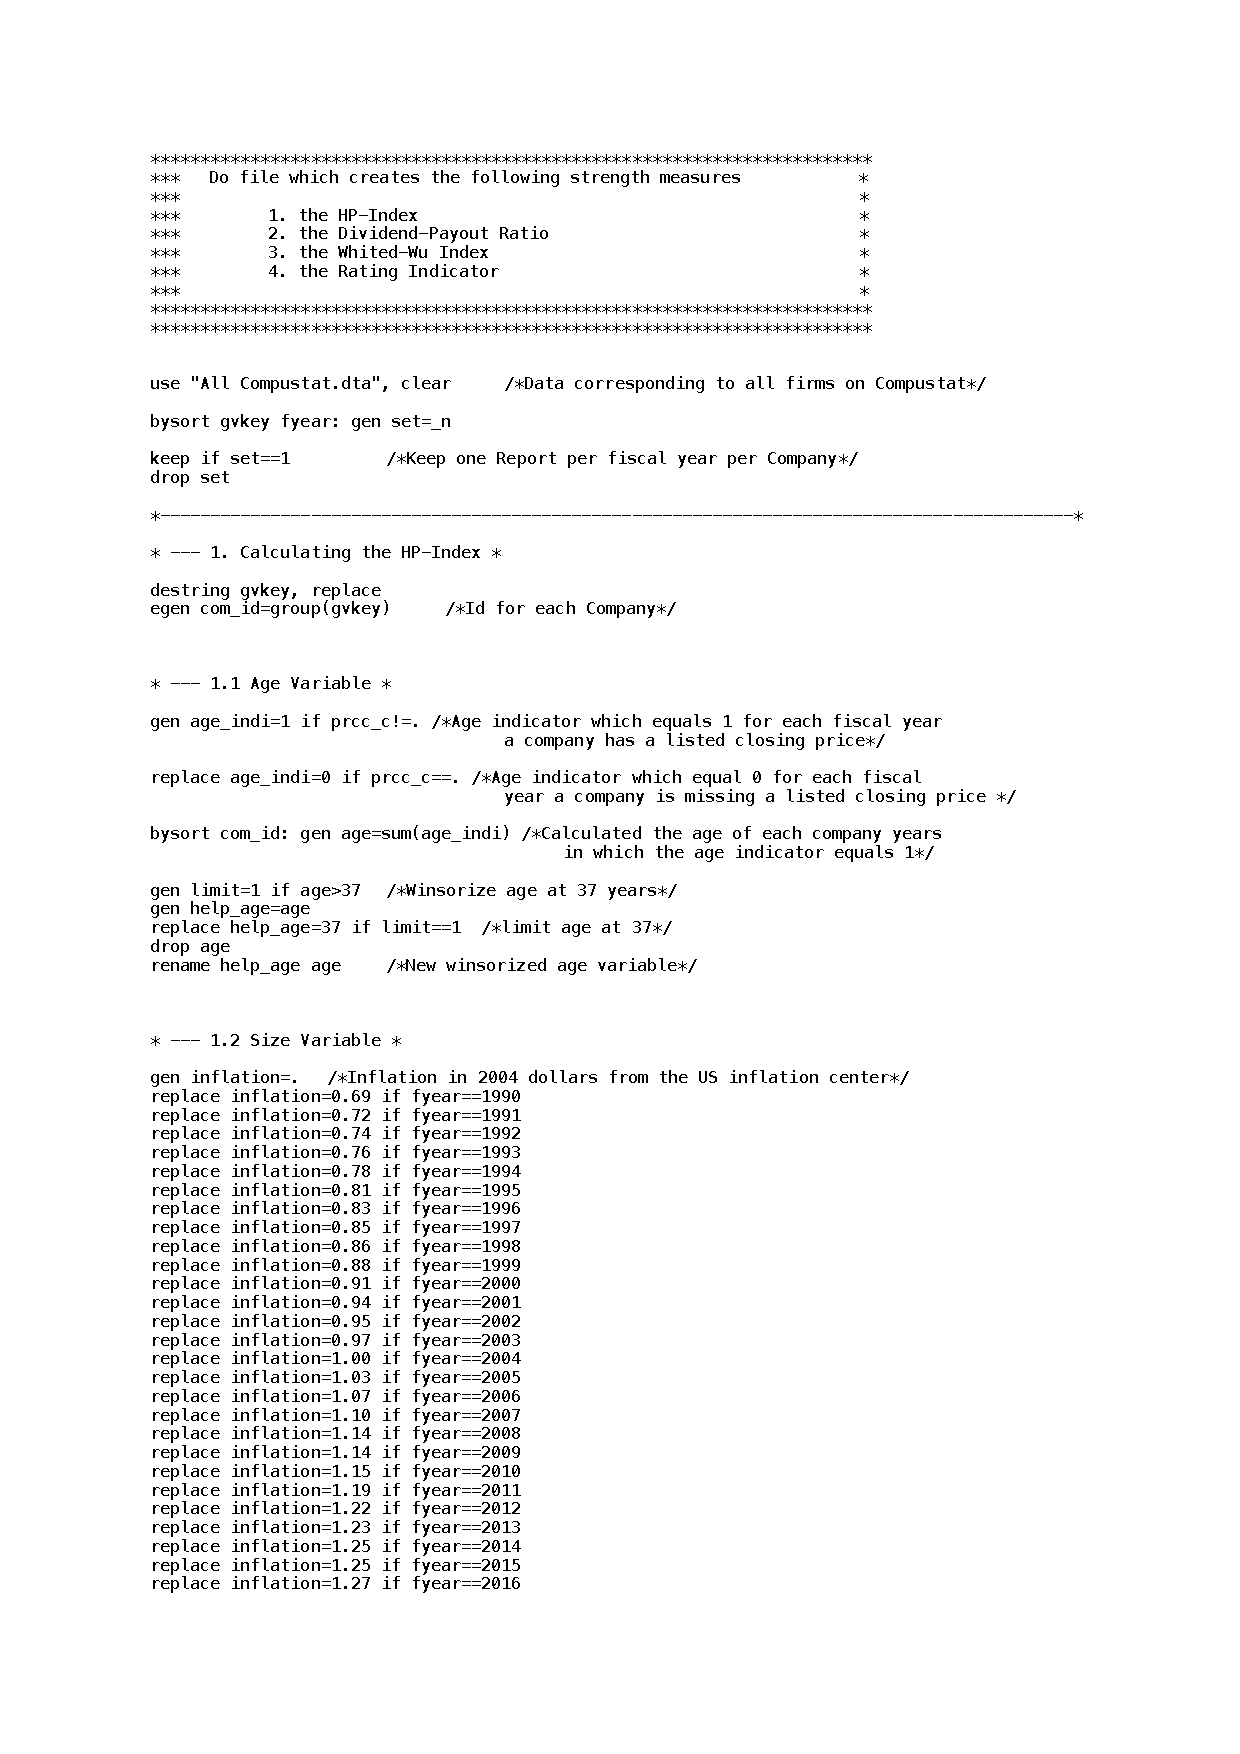
\includepdf[pages={1-3}]{SM_Thesis_copy.pdf}
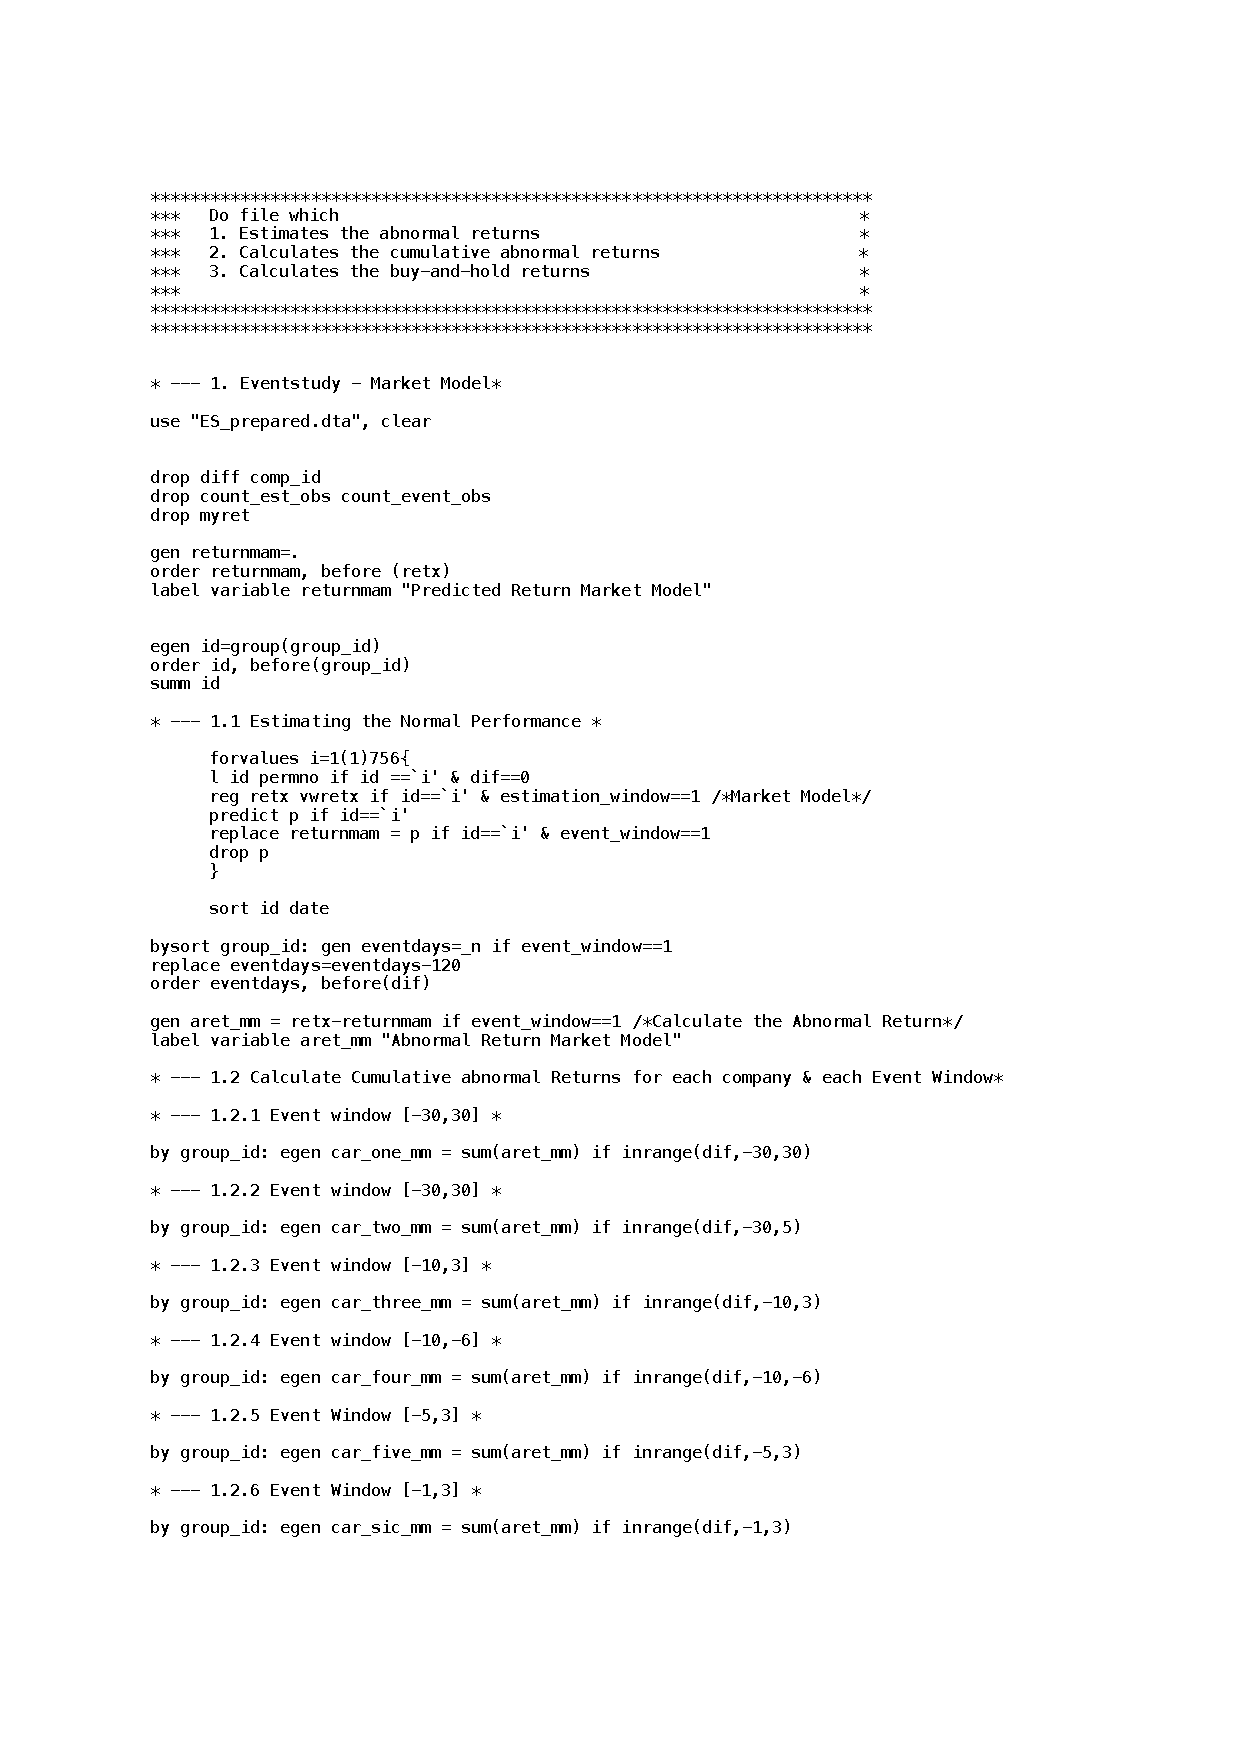
\includepdf[pages={1-3}]{ES_Thesis_copy.pdf}

\end{appendices}
\section*{Declaration of Authorship}
"I hereby declare 
\begin{itemize}
	\item that I have written thist hesis without any help fromothers and without the use of documents and aids other than those stated above;
	\item that I have mentioned all the sources used and that I have cited them correctly	according to established academic citation rules;
	\item that I have acquired any immaterial rights to materials I may have used such as images or graphs, or that I have produced such materials myself;
	\item that the topic or parts of it are not already the object of any work or examination of another course unless this has been explicitly agreed on with the faculty member in advance and is referred to in the thesis; 
	\item that I will not pass on copies of this work to third parties or publish them without the University’s written consent if a direct connection can be established with the University of St.Gallen or its faculty members;
	\item that I am aware that my work can be electronically checked for plagiarism and that I hereby grant the University of St.Gallen copyright in accordance with the Examination Regulations in so far as this is required for administrative action
	\item that I am aware that the University will prosecute any infringement of this declaration of authorship and, in particular, the employment of a ghostwriter, and that any such infringement may result in disciplinary and criminal consequences which may result in my expulsion from the University or my being stripped of my degree.”
\end{itemize} 

Date and Signature: \hrulefill

\hspace*{0mm}\phantom{Date and Signature: }Leopold Ingenohl\par
\vspace{0.5cm}
\noindent\small By submitting this academic term paper, I confirm through my conclusive action that I am submitting the Declaration of Authorship, that I have read and understood it, and that it is true.

\end{document}

